% A LaTeX template for MSc Thesis submissions to 
% Politecnico di Milano (PoliMi) - School of Industrial and Information Engineering
%
% S. Bonetti, A. Gruttadauria, G. Mescolini, A. Zingaro
% e-mail: template-tesi-ingind@polimi.it
%
% Last Revision: October 2021
%
% Copyright 2021 Politecnico di Milano, Italy. NC-BY

\documentclass[10pt]{Configuration_Files/PoliMi3i_thesis}

%------------------------------------------------------------------------------
%	REQUIRED PACKAGES AND  CONFIGURATIONS
%------------------------------------------------------------------------------

% CONFIGURATIONS
\usepackage{parskip} % For paragraph layout
\usepackage{setspace} % For using single or double spacing
\usepackage{emptypage} % To insert empty pages
\usepackage{multicol} % To write in multiple columns (executive summary)
\setlength\columnsep{15pt} % Column separation in executive summary
\setlength\parindent{0pt} % Indentation
\raggedbottom  
\usepackage{geometry}
\usepackage[dvipsnames]{xcolor} 

% NEURAL NETWORK GRAPH
\usepackage{amsmath} % for aligned
\usepackage{tikz}
\usepackage{listofitems} % for \readlist to create arrays
\usetikzlibrary{arrows.meta} % for arrow size
\usepackage[outline]{contour} % glow around text
\contourlength{1.4pt}
\tikzset{>=latex} % for LaTeX arrow head
\usepackage{xcolor}
\colorlet{myred}{red!80!black}
\colorlet{myblue}{blue!80!black}
\colorlet{mygreen}{green!60!black}
\colorlet{myorange}{orange!70!red!60!black}
\colorlet{mydarkred}{red!30!black}
\colorlet{mydarkblue}{blue!40!black}
\colorlet{mydarkgreen}{green!30!black}
\tikzstyle{node}=[thick,circle,draw=myblue,minimum size=22,inner sep=0.5,outer sep=0.6]
\tikzstyle{node in}=[node,green!20!black,draw=mygreen!30!black,fill=mygreen!25]
\tikzstyle{node hidden}=[node,blue!20!black,draw=myblue!30!black,fill=myblue!20]
\tikzstyle{node convol}=[node,orange!20!black,draw=myorange!30!black,fill=myorange!20]
\tikzstyle{node out}=[node,red!20!black,draw=myred!30!black,fill=myred!20]
\tikzstyle{connect}=[thick,mydarkblue] %,line cap=round
\tikzstyle{connect arrow}=[-{Latex[length=4,width=3.5]},thick,mydarkblue,shorten <=0.5,shorten >=1]
\tikzset{ % node styles, numbered for easy mapping with \nstyle
  node 1/.style={node in},
  node 2/.style={node hidden},
  node 3/.style={node out},
}
\def\nstyle{int(\lay<\Nnodlen?min(2,\lay):3)} % map layer number onto 1, 2, or 3

\definecolor{cadetgrey}{rgb}{0.5, 0.5, 0.5}

% PACKAGES FOR TITLES
\usepackage{titlesec}
% \titlespacing{\section}{left spacing}{before spacing}{after spacing}
\titlespacing{\section}{0pt}{3.3ex}{2.2ex}
\titlespacing{\subsection}{0pt}{3.3ex}{1.65ex}
\titlespacing{\subsubsection}{0pt}{3.3ex}{1ex}
\usepackage{color}

% PACKAGES FOR LANGUAGE AND FONT
\usepackage[english]{babel} % The document is in English  
\usepackage[utf8]{inputenc} % UTF8 encoding
\usepackage[T1]{fontenc} % Font encoding
\usepackage[11pt]{moresize} % Big fonts
\usepackage[bottom]{footmisc}

% PACKAGES FOR IMAGES
\usepackage{graphicx}
\usepackage{wrapfig}
\usepackage{transparent} % Enables transparent images
\usepackage{eso-pic} % For the background picture on the title page
\usepackage{subfig} % Numbered and caption subfigures using \subfloat.
\usepackage{tikz} % A package for high-quality hand-made figures.
\usetikzlibrary{}
\graphicspath{{./Images/}} % Directory of the images
\usepackage{caption} % Coloured captions
\usepackage{xcolor} % Coloured captions
\usepackage{amsthm,thmtools,xcolor} % Coloured "Theorem"
\usepackage{float}

% STANDARD MATH PACKAGES
\usepackage{amsmath}
\usepackage{amsthm}
\usepackage{verbatim}
\usepackage{amssymb}
\usepackage{amsfonts}
\usepackage{bm}
\usepackage[overload]{empheq} % For braced-style systems of equations.
\usepackage{fix-cm} % To override original LaTeX restrictions on sizes

% PACKAGES FOR TABLES
\usepackage{tabularx}
\usepackage{longtable} % Tables that can span several pages
\usepackage{colortbl}

% PACKAGES FOR ALGORITHMS (PSEUDO-CODE)
\usepackage{algorithm}
\usepackage{algorithmic}

% PACKAGES FOR REFERENCES & BIBLIOGRAPHY
\usepackage[colorlinks=true,linkcolor=black,anchorcolor=black,citecolor=black,filecolor=black,menucolor=black,runcolor=black,urlcolor=black]{hyperref} % Adds clickable links at references
\usepackage{cleveref}
\usepackage[square, numbers, sort&compress]{natbib} % Square brackets, citing references with numbers, citations sorted by appearance in the text and compressed
\bibliographystyle{abbrvnat} % You may use a different style adapted to your field

% OTHER PACKAGES
\usepackage{pdfpages} % To include a pdf file
\usepackage{afterpage}
\usepackage{lipsum} % DUMMY PACKAGE
\usepackage{fancyhdr} % For the headers
\fancyhf{}
\usepackage{optidef}
\usepackage{array}

\usepackage{tikz}
\newcommand*{\mycirc}[1]{\tikz {\node at (0,0) [inner sep=0] {};\fill (0,0.5ex) circle (#1);}}
\newcommand\sbullet[1][.5]{\mathbin{\vcenter{\hbox{\scalebox{#1}{$\bullet$}}}}}

% Input of configuration file. Do not change config.tex file unless you really know what you are doing. 
\input{Configuration_Files/config}

%----------------------------------------------------------------------------
%	NEW COMMANDS DEFINED
%----------------------------------------------------------------------------

% EXAMPLES OF NEW COMMANDS
\newcommand{\bea}{\begin{eqnarray}} % Shortcut for equation arrays
\newcommand{\eea}{\end{eqnarray}}
\newcommand{\e}[1]{\times 10^{#1}}  % Powers of 10 notation

%----------------------------------------------------------------------------
%	ADD YOUR PACKAGES (be careful of package interaction)
%----------------------------------------------------------------------------

%----------------------------------------------------------------------------
%	ADD YOUR DEFINITIONS AND COMMANDS (be careful of existing commands)
%----------------------------------------------------------------------------

%----------------------------------------------------------------------------
%	BEGIN OF YOUR DOCUMENT
%----------------------------------------------------------------------------
\geometry{a4paper, top=2.5cm, bottom=2.5cm, left=2.5cm, right=2.5cm} 

\begin{document}

\newcommand{\U}{\mathbb{U}}
\newcommand{\N}{\mathbb{N}}
\renewcommand{\S}{\mathbb{S}}
\newcommand{\E}{\mathcal{E}}
\fancypagestyle{plain}{%
\fancyhf{} % Clear all header and footer fields
\fancyhead[RO,RE]{\thepage} %RO=right odd, RE=right even
\renewcommand{\headrulewidth}{0pt}
\renewcommand{\footrulewidth}{0pt}}

\newcolumntype{C}[1]{>{\centering\arraybackslash}p{#1}}
%----------------------------------------------------------------------------
%	TITLE PAGE
%----------------------------------------------------------------------------
\let\cleardoublepage=\clearpage
\pagestyle{empty} % No page numbers
%\frontmatter % Use roman page numbering style (i, ii, iii, iv...) for the preamble pages


\puttitle{
	title=RESEARCH PROJECT\\ \\
	\Large{Dynamics in a time-discrete food-chain model with strong pressure on preys\\}, % Title of the thesis
	name = Lorenzo Ferrara \vspace{0.5 cm}\\ 
	       \hspace*{2.42 cm}Sofia Raschi, 
	course=Quantitative and Qualitative Methods in Dynamical Systems, % Study Programme (in Italian)
	%ID  = ,  % Student ID number (numero di matricola)
	Professor = Pau Martin De La Torre - Inmaculada Baldoma Barraca, 
	academicyear={2022-23},  % Academic Year
} % These info will be put into your Title page 

%----------------------------------------------------------------------------
%	PREAMBLE PAGES: ABSTRACT (inglese e italiano), EXECUTIVE SUMMARY
%----------------------------------------------------------------------------

%\setcounter{page}{1} % Set page counter to 1
% ABSTRACT IN ENGLISH
%\chapter*{Abstract} 
%\thispagestyle{empty}
%\AddToShipoutPicture*{\BackgroundPic}
%\clearpage

% TABLE OF CONTENTS
\pagenumbering{arabic}
\tableofcontents % Table of contents 
\pagenumbering{}

%-------------------------------------------------------------------------
%	THESIS MAIN TEXT
%-------------------------------------------------------------------------
% In the main text of your thesis you can write the chapters in two different ways:
%
%(1) As presented in this template you can write:
%    \chapter{Title of the chapter}
%    *body of the chapter*
%
%(2) You can write your chapter in a separated .tex file and then include it in the main file with the following command:
%    \chapter{Title of the chapter}
%    \input{chapter_file.tex}
%
% Especially for long thesis, we recommend you the second option.

%\addtocontents{toc}{\vspace{2em}} % Add a gap in the Contents, for aesthetics
\mainmatter % Begin numeric (1,2,3...) page numbering

% --------------------------------------------------------------------------
% NUMBERED CHAPTERS % Regular chapters following
% --------------------------------------------------------------------------

\chapter{Introduction}
\label{ch:}

This project aims to examine a discrete-time dynamical system that models the population dynamics of three interacting species $x$, $y$ and $z$, with non-overlapping generations. Specifically, $x$ represents the prey, $y$ represents the predator that preys on $x$, and $z$ represents the top-predator, which preys on $y$ and also interferes with the reproduction of $x$. Additionally, $x$ also interferes with its own growth. These interactions are summarized in the next \autoref{fig:Scheme}. 

\begin{figure}[h]
\centering
   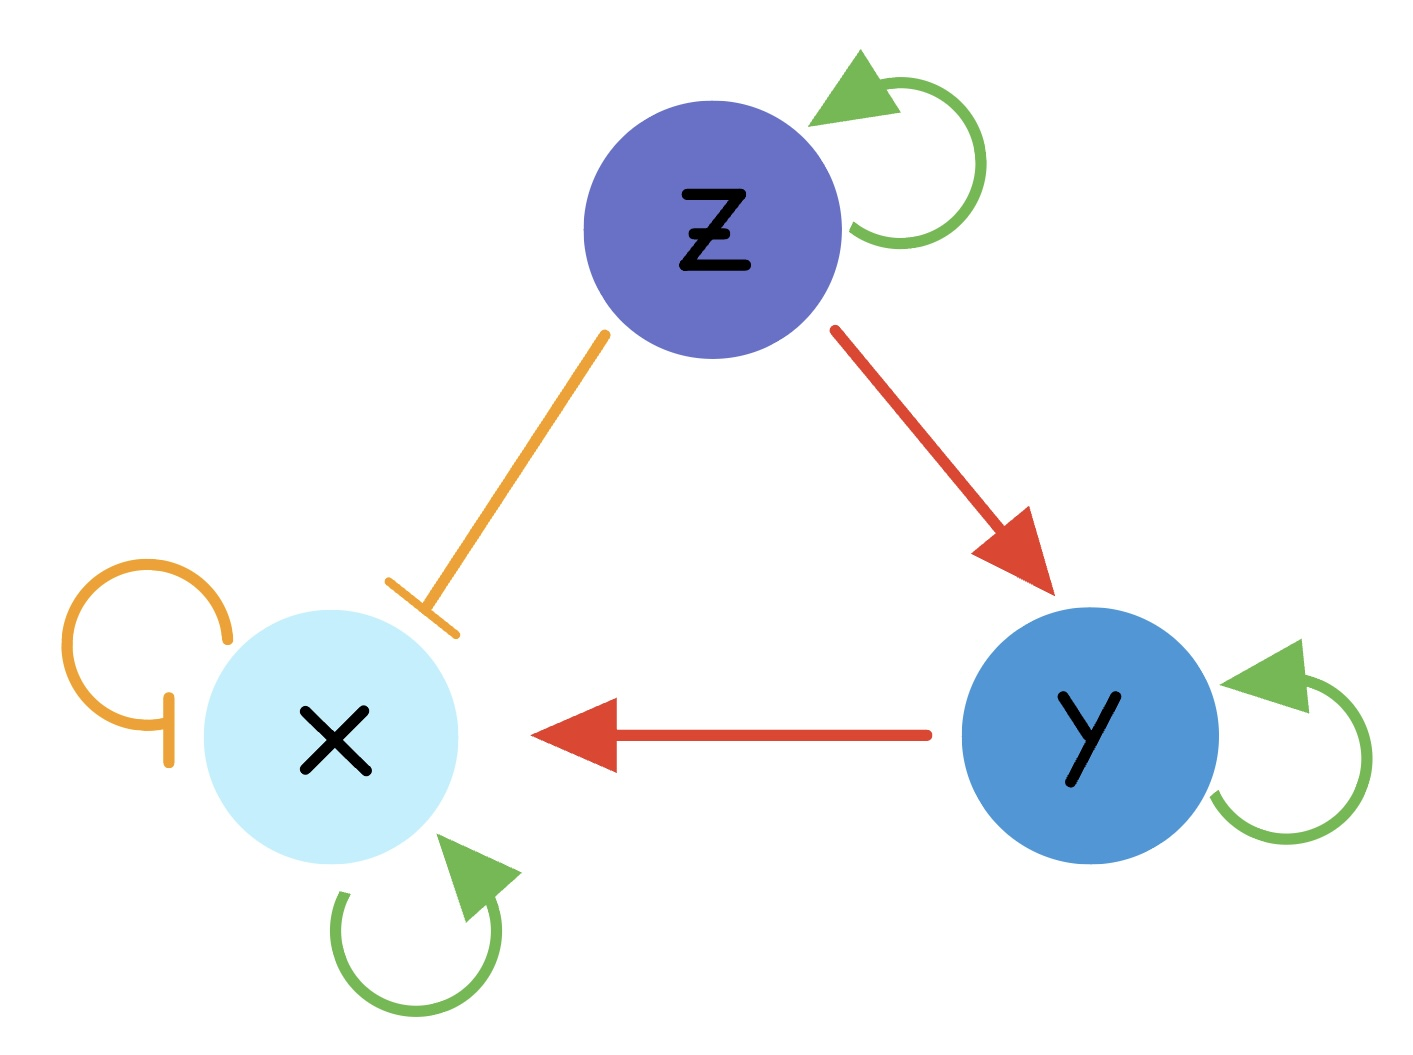
\includegraphics[scale=0.10]{images/Chapter 1/prey_pred.jpg} 
   \caption{Food-chain scheme}
   \label{fig:Scheme}
\end{figure}

An example of this ecosystem in nature involves a population of small mammals ($x$) as prey, a population of snakes ($y$) as primary predators, and a population of birds of prey ($z$) as top predators. The small mammal population can increase exponentially in the absence of predators, but is limited by the availability of food and by interference from the birds of prey. The snake population, in turn, is limited by the availability of small mammals and is also impacted by predation from the birds. The bird of prey population is limited by the availability of snakes, moreover, it interferes with the survival rate of small mammals, for example, they may scare them away from food or shelter. This interference can have cascading effects throughout the ecosystem, leading to changes in the abundance and distribution of the different species.

To analyze this system, we will examine the conditions that lead to species extinction and those that result in stabilization on periodic orbits, using advanced mathematical techniques. This involves studying the stability of equilibrium points, or the existence and stability of periodic solutions.
We also use numerical methods to simulate the dynamics of the system and study its behaviour under different initial conditions and parameter values. Overall, this project will provide a deeper understanding of how complex ecological interactions between multiple species can lead to extinction or stabilization.


\chapter{Mathematical model}
\label{ch:}
This ecosystem can be described through the following discrete-time system:
\begin{equation}
  \begin{pmatrix} x_{n+1}\\y_{n+1}\\z_{n+1}
\end{pmatrix}
=
\begin{pmatrix} \mu x_n (1-x_n-y_n-z_n)\\ \beta y_n (x_n - z_n)\\ \gamma y_n z_n
\end{pmatrix}
= T
\begin{pmatrix} x_{n}\\y_{n}\\z_{n}
\end{pmatrix}
\label{eq:eq1}
\end{equation}

where $x$, $y$ and $z$ represent the normalised population densities. These quantities must be positive and their sum must be at most 1, so the domain is defined as: 
\begin{center}
  $ \mathbb{U} = \{ \left ( x,y,z \right ) \in \mathbb{R}^3: x,y,z \ge 0 \hspace{5pt} \wedge \hspace{5pt} x+y+z \le 1 \} $ .
\end{center}

The parameters $\mu$, $\beta$ and $\gamma$ are positive constants representing the reproduction rates of each population. We will limit our analysis to a specific set of parameters: 
\begin{center}
 $Q = \{ \left (\mu, \beta, \gamma \right) \in \left (0,4 \right] \times \left [2.5,5 \right ]\times \left [5,9.4 \right ] \}$ .
\end{center}
which will allow us to study important phenomena such as cascade extinctions and periodic orbits.

Our goal is to investigate the conditions that lead to extinction. To begin with, we will analyse the particular point $(0,0,0)$, which corresponds to the extinction of all three species. This can be achieved in just one iteration starting from the points $(1,0,0), \{ (0,y,0) \in \mathbb{U} \}$ and  $\{(0,0,z) \in \mathbb{U} \}$, by applying the map T once.

The extinction of all three species can also occur in other situations. Mathematically, this occurs whenever the orbits move outside of the domain $\mathbb{U}$. 
From a biological point of view, the domain $\mathbb{U}$ states that the carrying capacity K=1 cannot be surpassed and that all the population densities must be non-negative. 
% nella realtà perchè si estinguono?

%Now, we want to define a set which is well-defined for all iterates of the system \ref{eq:eq1}, we reduce this set to $\mathcal{E} = \{(x,0,z) \in \mathbb{U}\} \cup \{(x,y,z)\in \mathbb{U}: y > 0 \wedge x \ge z\}$

We want to define the invariant set $\mathbb{S}$ as the set of points whose orbits will always remain inside the domain $\mathbb{U}$. To do so, we first define the one-step escaping set $\Theta$ and the escaping set $\Gamma$, the sets of the points which end up out of the domain in one step and which will eventually come out.
\begin{center}
  $\Theta=\{ (x, y, z)\in\U: T(x,y,z)\notin \U\} $
\end{center}
\begin{center}
  $\Gamma = \bigcup\limits_{n\in\mathbb{N}} T^{-n}(\Theta)$.  
\end{center}

In this way, it's easy to define $\S$ as $\S = \U \textbackslash \Gamma$.
However, it can be difficult to study the behaviour of this system in the entire domain $\U$, and it is useful to notice that by restricting our analysis to the set $$\E = \{(x,0,z) \in \mathbb{U}\} \cup \{(x,y,z)\in \mathbb{U}: y > 0 \wedge x \ge z\}$$ we can study a smaller and simpler portion of space without losing the relevant information. In fact, it can be proven that $\S\subset\E\subset\U$, so all the phenomena we want to study in S are guaranteed to occur inside $\E$.

To illustrate the complexity of studying the region S, we provide an example showing the amount of time it takes for a given system, with an initial condition in the plane $z=0$, to exceed the carrying capacity and go extinct (as shown in \autoref{fig:Iterations}).
\\
The color gradient indicates the number of iterations required for the orbit to leave S, with 1 iteration represented by blue and 20 iterations represented by yellow.

\begin{figure}[h]
\centering
    \begin{tabular}{cc}
    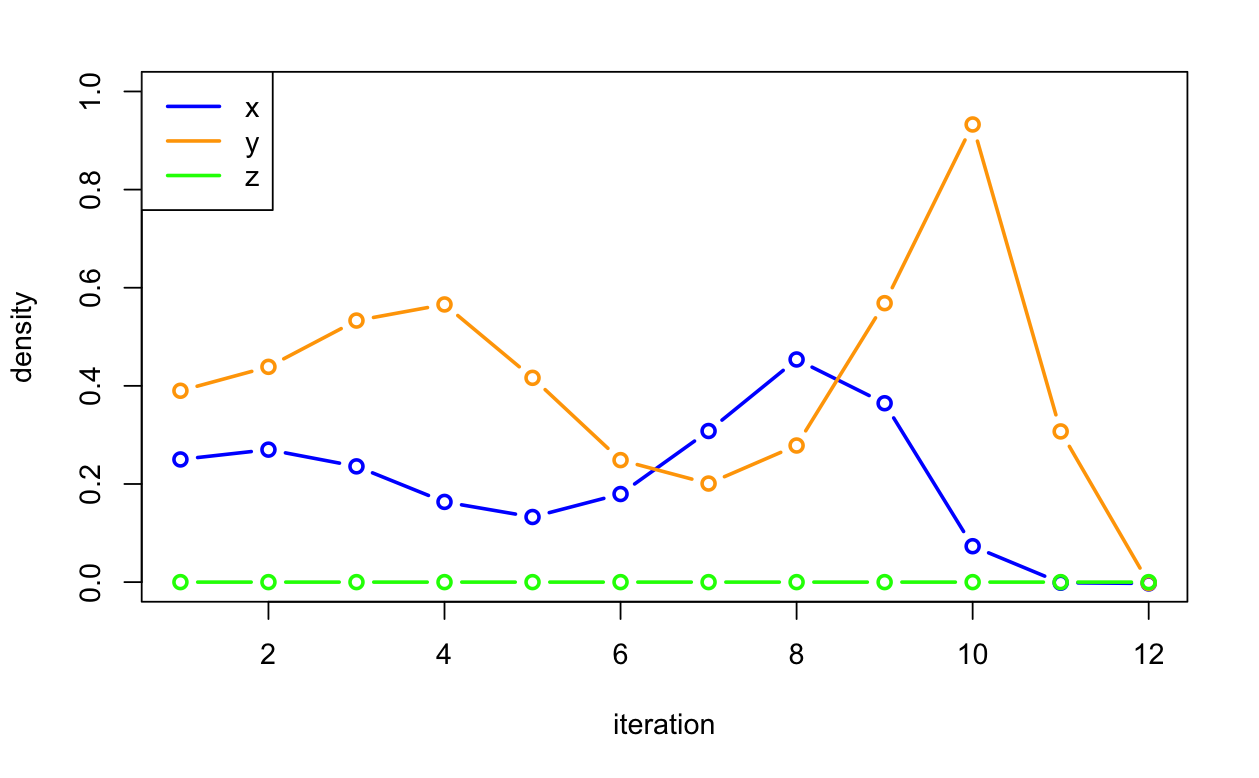
\includegraphics[width=0.45\linewidth]{images/Chapter 2/linee1.png} &
    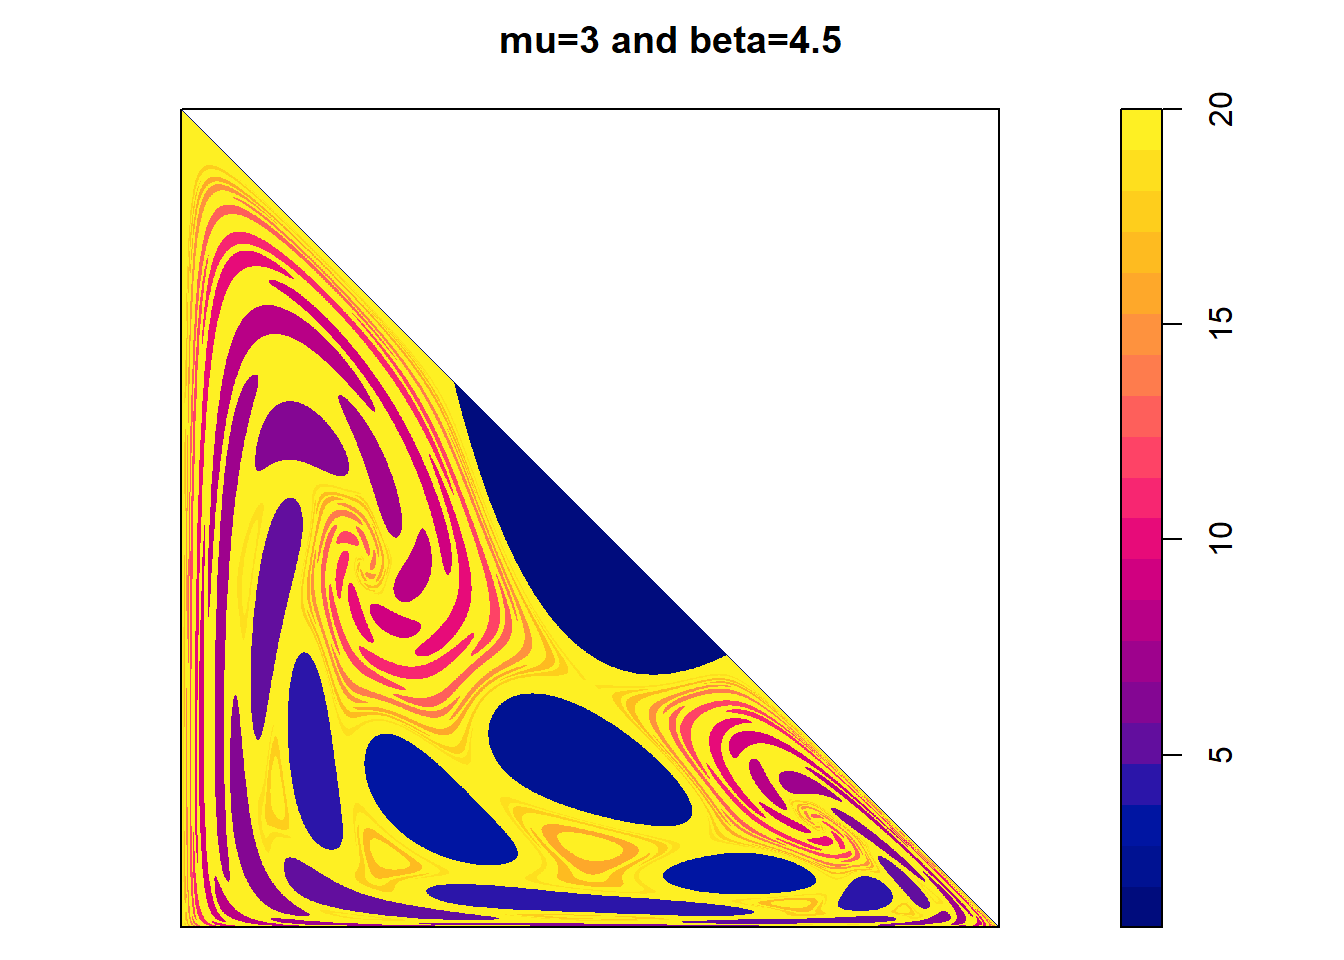
\includegraphics[width=0.45\linewidth]{images/Chapter 2/unnamed-chunk-4-1.png} &
     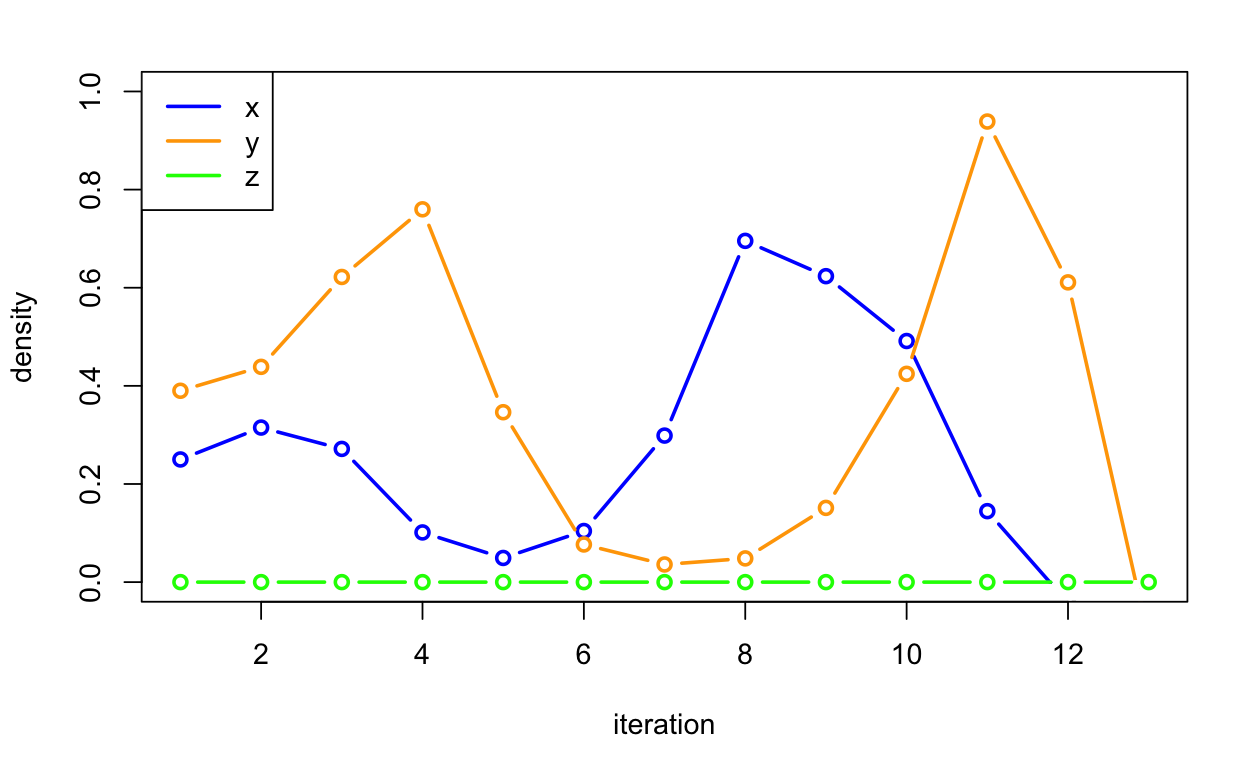
\includegraphics[width=0.45\linewidth]{images/Chapter 2/linee2.png} &
    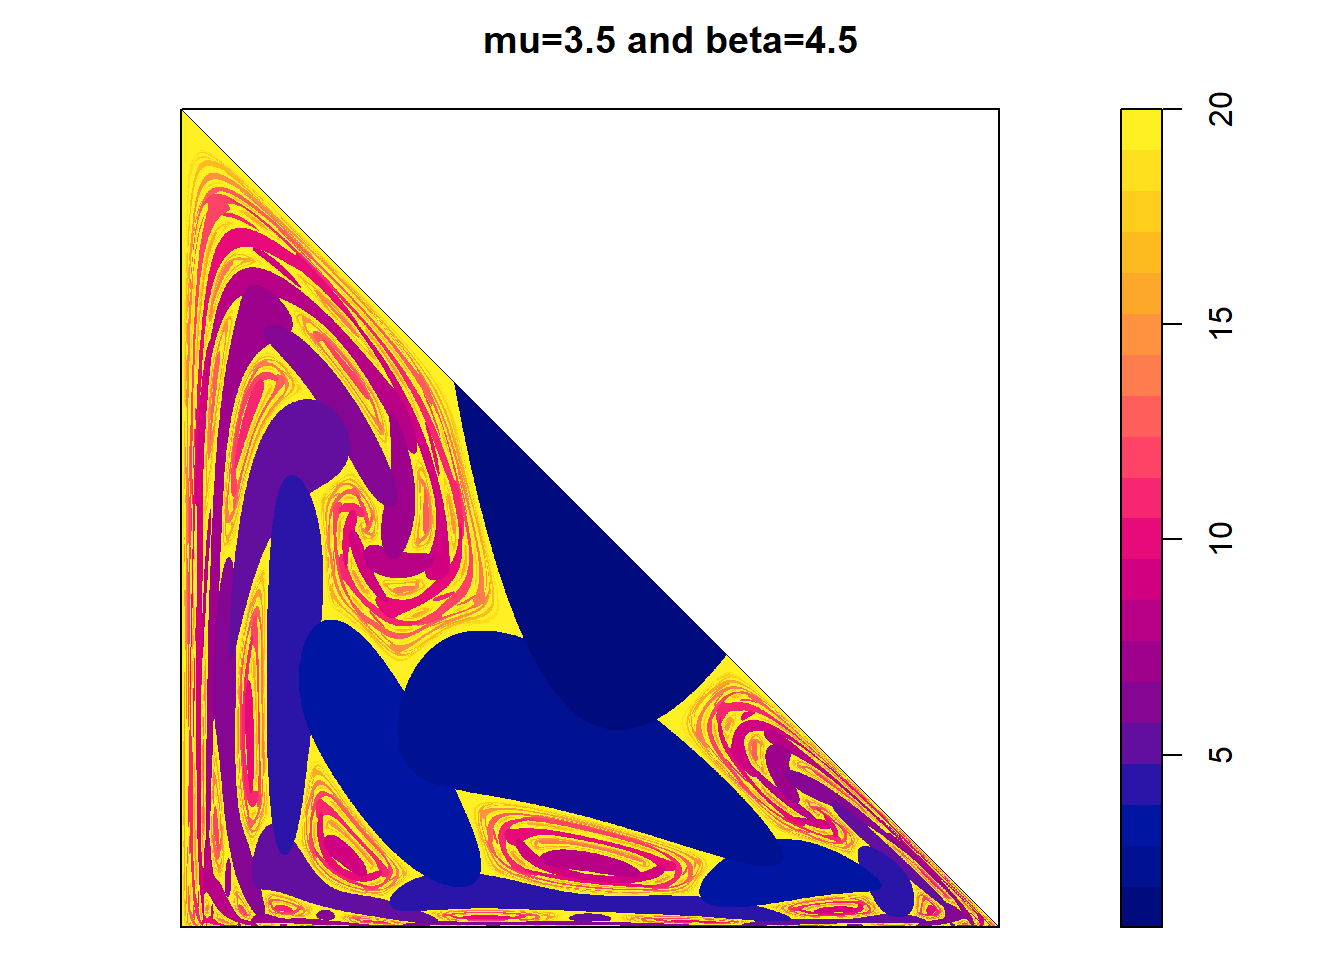
\includegraphics[width=0.45\linewidth]{images/Chapter 2/unnamed-chunk-6-1.png} &
    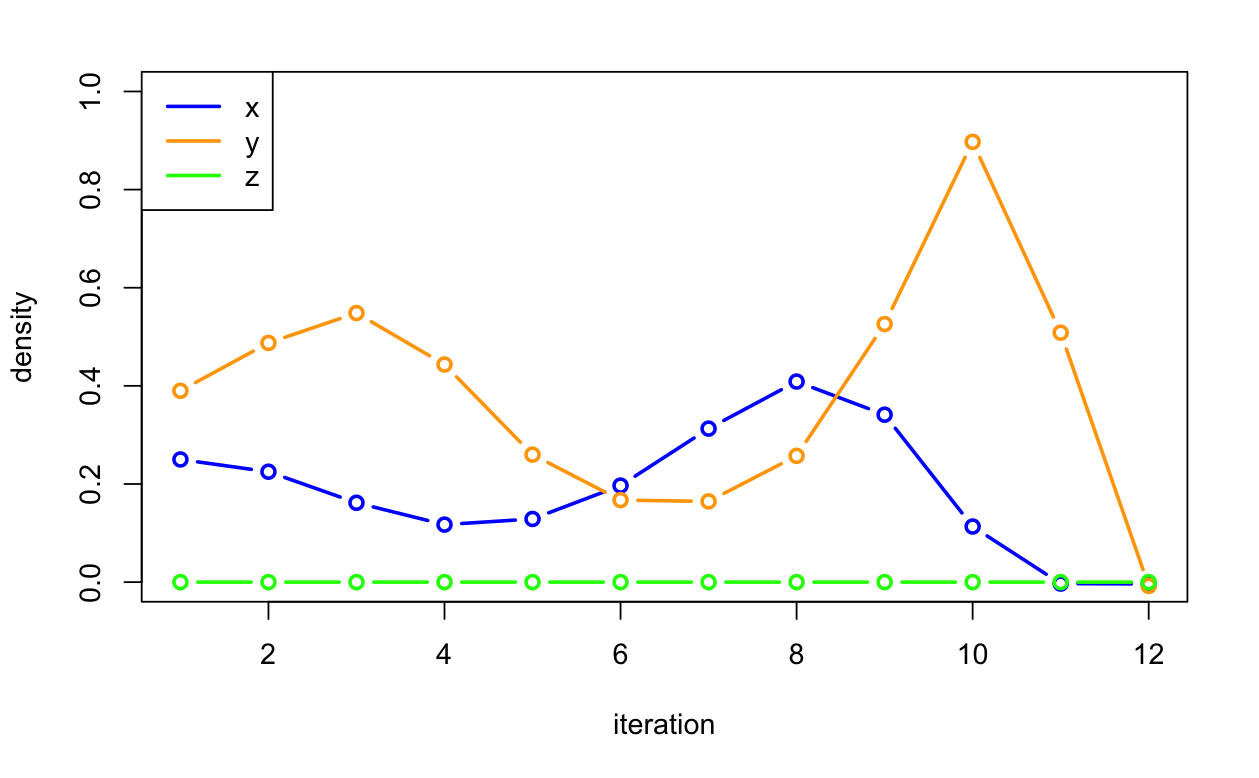
\includegraphics[width=0.45\linewidth]{images/Chapter 2/linee3.png} &
    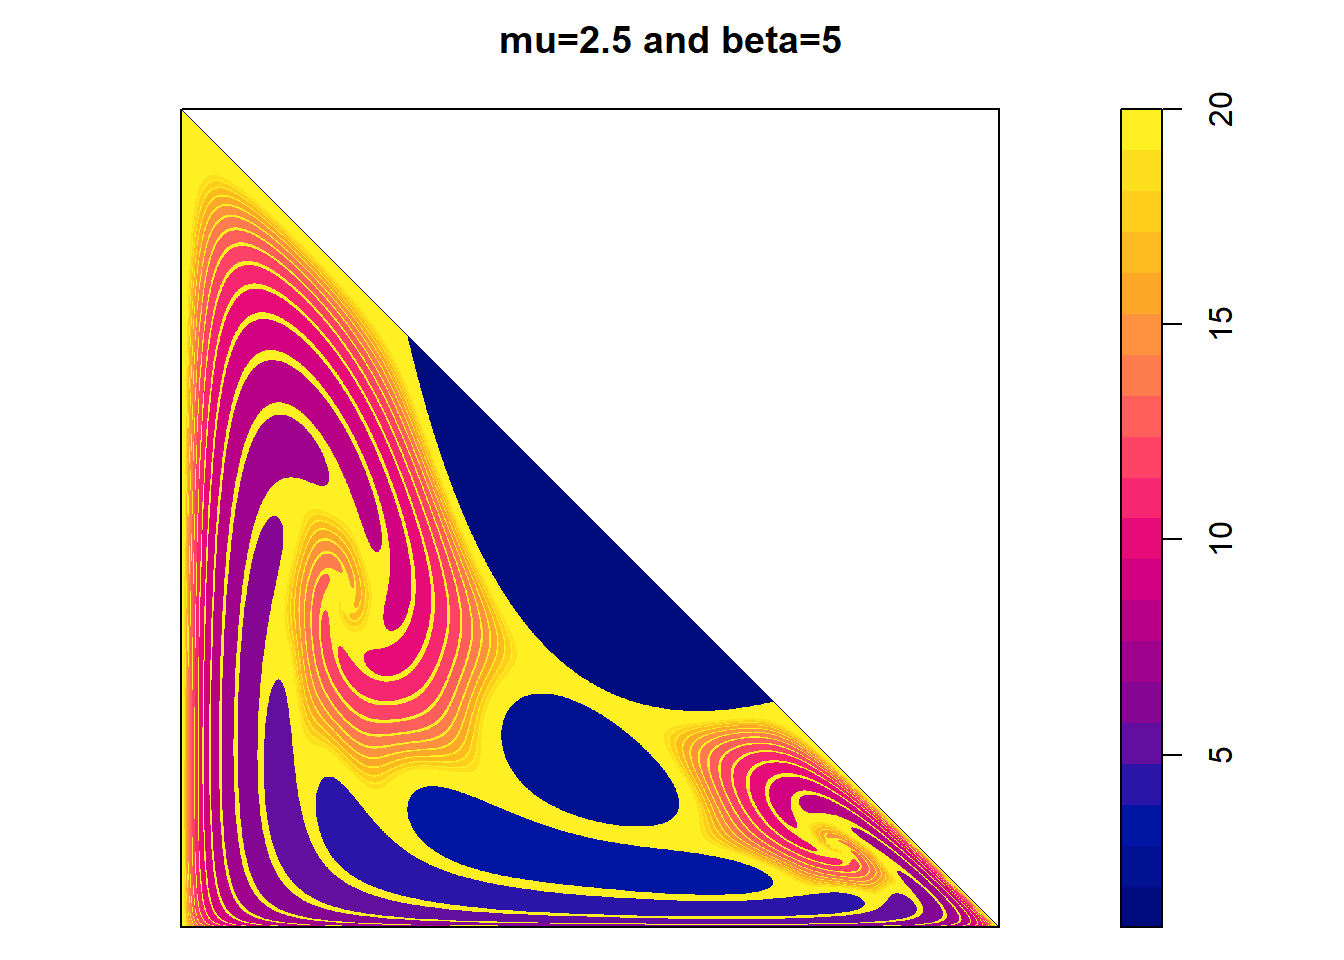
\includegraphics[width=0.45\linewidth]{images/Chapter 2/unnamed-chunk-8-1.png}
    \end{tabular}
    \caption{Time-series and escaping times for $(\mu, \beta) = (3, 4.5)$, $(3.5, 4.5)$ and $(2.5, 5)$}
    \label{fig:Iterations}
\end{figure}

\chapter{Analysis of the fixed points}

\section{Computation of the fixed points}

Let's first compute the fixed points of the system. 
\begin{eqnarray}
x & = & \mu x (1-x-y-z) \label{eq:sys1}\\
y & = & \beta y (x-z) \label{eq:sys2}\\
z & = & \gamma y z \label{eq:sys3}
\end{eqnarray}

We start from \autoref{eq:sys3}, the solutions of this equation are either $z=0$ or $y=\frac{1}{\gamma}$.
\begin{itemize}
  \item if $z=0$: the system becomes 
  \begin{eqnarray}
    x & = & \mu x (1-x-y-z) \label{eq:sys11}\\
    y & = & \beta y (x-z) \label{eq:sys22} \\
    0 & = & 0 \label{eq:sys33}
    \end{eqnarray}

  Now look at \autoref{eq:sys22}, the feasible solutions are $y=0$ and $y=\frac{1}{\gamma}$.
  \begin{itemize}
     \item if $y=0$: we need to solve just $ x  = \mu x (1-x) $, which has the following solutions 
     \begin{equation*}
        \begin{cases}
      x=0 \\ 
      x = \frac{\mu-1}{\mu}
        \end{cases}
     \end{equation*}
     So we find two fixed points $P_1 = (0,0,0)$ and $P_2 = (\frac{\mu-1}{\mu}, 0, 0)$.
     \item if $x= \frac{1}{\beta}$: the system becomes 
     \begin{eqnarray}
    \frac{1}{\beta} & = & \frac{\mu}{\beta} (1-\frac{1}{\beta}-y) \\
    y & = & y \\
    0 & = & 0
    \end{eqnarray}
    which is satisfied for $y=1-\frac{1}{\beta}-\frac{1}{\mu}$, so we compute another fixed point $P_3 = (\frac{1}{\beta}, 1-\frac{1}{\mu}-\frac{1}{\beta}, 0)$.
    \end{itemize}
  
    \item if $y=\frac{1}{\gamma}$: the system is 
    \begin{eqnarray}
    x & = &  \mu x (1-x-\frac{1}{\gamma}-z) \label{eq:sys44}\\
    \frac{1}{\gamma} & = & \frac{\beta}{\gamma} (x-z) \label{eq:sys55}\\
    z & = & z
    \end{eqnarray}
    We substitute the expression of $z$ obtained from \ref{eq:sys55}, which is $z = x - \frac{1}{\beta}$, into \ref{eq:sys44}, obtaining 
    \begin{equation*}
        \begin{cases}
      x=0 \\ 
      x = \frac{1}{2} ( 1-\frac{1}{\mu}+\frac{1}{\beta}-\frac{1}{\gamma})
        \end{cases}
     \end{equation*}
     So we find  the fixed points $P_4 = (\frac{1}{2}(1-\frac{1}{\mu}+\frac{1}{\beta}-\frac{1}{\gamma}), \frac{1}{\gamma}, \frac{1}{2}(1-\frac{1}{\mu}-\frac{1}{\beta}-\frac{1}{\gamma})$ and   $P_5 = (0, \frac{1}{\gamma}, -\frac{1}{\beta})$.

\end{itemize}

Summing up, the fixed points are:
\begin{itemize}
\item[\mycirc{2pt}] $P_1 = (0,0,0)$
\item[\mycirc{2pt}] $P_2 = (\frac{\mu-1}{\mu}, 0, 0)$
\item[\mycirc{2pt}] $P_3 = (\frac{1}{\beta}, 1-\frac{1}{\mu}-\frac{1}{\beta}, 0)$
\item[\mycirc{2pt}] $P_4 = (\frac{1}{2}(1-\frac{1}{\mu}+\frac{1}{\beta}-\frac{1}{\gamma}), \frac{1}{\gamma}, \frac{1}{2}(1-\frac{1}{\mu}-\frac{1}{\beta}-\frac{1}{\gamma}))$
\end{itemize}  
We notice that  $P_5 = (0, \frac{1}{\gamma}, -\frac{1}{\beta})$ has a negative coordinate and, since we're dealing with densities, it is not biologically meaningful, so we exclude it from our analysis.

\section{Existence and analysis of the fixed points}

Let's now analyse how many of the fixed points of the system are contained in our domain of interest $\E$, as the reproduction rates $\mu, \beta, \gamma$ vary in $Q$.

To study the stability of the fixed points, the Jacobian matrix has been used: 

$$J(x,y,z) = \begin{pmatrix} \mu(1-2x-y-z) & -\mu x & -\mu x \\ \beta y & \beta(x-z) & -\beta y \\ 0 & \gamma z & \gamma y
\end{pmatrix} $$

\subsection{$P_1 = (0,0,0)$}
$P_1$ doesn't depend on any parameter, it is always contained in $\E$. Indeed, as mentioned before, this fixed point represents the extinction of the three species, which can take place for any value of $(\mu,\beta,\gamma)\in Q$.

After studying the Jacobian matrix, we can analyze $P_1$:
\begin{itemize}
\item for $\mu = 1$ it is non-hyperbolic, as expected, since $P_1$ and $P_2$ coincide in this particular case.
\item for $0 < \mu < 1$ it is a locally asymptotically stable sink node; indeed, biologically speaking, $\mu<1$ indicates that not only there's no growth, but also the prey population is decreasing.  
\item for $\mu > 1$ it is a saddle with an unstable invariant manifold of dimension 1, locally tangent to the x-axis.
\end{itemize}

\subsection{$P_2 = (\frac{\mu-1}{\mu}, 0, 0)$}

$P_2$ is contained in $\E$ for $\mu\geq 1$, this is also intuitive from a biological point of view since at each iteration, the new generation will have fewer individuals than the previous one, converging to 0. Furthermore, this fixed point can be reached if the two predator species have gone extinct and the dynamic is only governed by the logistic map of the prey $x$, that is $x_{n+1} = \mu x_n (1-x_n)$. \\
We can remind that for $\mu=1$, the first two fixed points coincide $P_1 \equiv P_2$, while for $\mu=\frac{\beta}{\beta-1}$ we notice $P_2 \equiv P_3$.\\
As regards stability, we identify three regions:
\begin{itemize}
    \item for $1 < \mu < \frac{\beta}{\beta-1}, \hspace{2} P_2$ is a locally asymptotically stable sink node.
    \item for $\frac{\beta}{\beta-1} < \mu < 3$ it is a saddle with an unstable invariant manifold of dimension 1, locally tangent to the x-axis.
    \item for $3 < \mu \le 4$ it is a saddle with an unstable invariant manifold of dimension 2.
\end{itemize}

\subsection{$P_3 = (\frac{1}{\beta}, 1-\frac{1}{\mu}-\frac{1}{\beta}, 0)$}

$P_3$ is contained in the domain $\E$ for $\mu\geq \frac{\beta}{\beta-1}\geq \frac{5}{4}$, that means $\beta \le 5$ and $\frac{1}{\mu} + \frac{1}{\beta} \le {1}$. \\ 
The biological meaning of this fixed point corresponds to the extinction of the top-predator and the survival of the prey and the predator. However, this point can be reached only when the initial conditions of the system are $(x,y,z) =(x_0,y_0,0)$, i.e. in an initial situation with no top predator. Indeed $z_n = \gamma y_{n-1} z_{n-1} = ... = \gamma^{n} (\prod\limits_{i=0}^{n-1} y_i ) z_0$ which can be 0 only in two cases:
\begin{itemize}
\item if $z_0=0$: in this case the 3-species system degenerates to a 2-species system, which has its fixed point when the two species have found a balance between hunting rate, growth rate, and the populations' dimensions.
\item if $\exists \,  \tilde{n}$ s.t. $y_{\tilde{n}}=0$. But in that case we'd have $y_n=0$ $\forall n\geq\tilde{n}$ and we're looking for points which have $y=1-\frac{1}{\mu}-\frac{1}{\beta}>0$, so we exclude this possibility.
\end{itemize} 

The point $P_3$ coincides with the point $P_4$ for $\mu=\frac{\beta \gamma}{(\beta-1)\gamma -\beta}$.

Analysing the Jacobian $J(P_3)$ we notice that it is a locally asymptotically stable sink node for $\frac{\beta}{\beta-1} < \mu < 2 \beta (\beta -1 - \sqrt{\beta(\beta -2)})$, while it is a locally asymptotically stable spiral node-sink for $2 \beta (\beta -1 - \sqrt{\beta(\beta -2)}) < \mu < \frac{\beta \gamma}{(\beta-1)\gamma -\beta}$. \\
For $\frac{\beta \gamma}{(\beta-1)\gamma -\beta} < \mu < min\{4, \frac{\beta}{\beta-2}\}$ the fixed point is an unstable spiral-sink node-source, while for $min\{4, \frac{\beta}{\beta-2}\} < \mu < 4$ it is an unstable spiral-node source


\subsection{$P_4 = (\frac{1}{2}(1-\frac{1}{\mu}+\frac{1}{\beta}-\frac{1}{\gamma}), \frac{1}{\gamma}, \frac{1}{2}(1-\frac{1}{\mu}-\frac{1}{\beta}-\frac{1}{\gamma})$}

$P_4$ is contained in $\E$ for $\frac{1}{\mu}+\frac{1}{\beta}+\frac{1}{\gamma}\leq 1$.\\
Let's define a function $\psi:[5,9.4]\to[\frac{\beta \gamma}{(\beta-1)\gamma -\beta},4)$, then the three species achieve a static coexistence equilibrium for $\frac{\beta \gamma}{(\beta-1)\gamma -\beta} < \mu < \psi(\beta,\gamma)$, since $P_4$ is a locally asymptotically stable spiral-sink. While for $ \psi(\beta,\gamma) < \mu \le 4$ it is an unstable spiral-source node-sink.


\chapter{Local bifurcations}
In order to summarize the results obtained in the previous chapter we need to identify different regions of the parameters inside which the behaviour of the fixed points does not change, so that we can define the biological evolution of the system inside those zones. The borders of these areas identify the local bifurcations. The mathematical relation between the intervals considered can be proven by comparing them.

\begin{itemize}
\item[A.] $0 < \mu < 1 \to $ the system has  $P_1$ as a unique fixed point, due to the fact that it is an asymptotically stable node in this region, all the species go to extinction.
\item[B.] $1 < \mu < \frac{\beta}{\beta-1} \to$ there exist two fixed points $P_1$ and $P_2$, The second one is asymptotically stable, so we notice that in this region only the prey survives, while the other two species go to extinction.
\item[C.] $ \frac{\beta}{\beta-1} < \mu < 2 \beta (\beta -1 - \sqrt{\beta(\beta -2)}) \to$ in this zone there are three fixed points $P_1, P_2$ and $P_3$. Since $P_3$ is the only one asymptotically stable, the top-predator goes to extinction.
\item[D.] $ 2 \beta (\beta -1 - \sqrt{\beta(\beta -2)}) < \mu <  \frac{\beta \gamma}{(\beta-1)\gamma-\beta} \to$ there exists three fixed points $P_1, P_2$ and $P_3$, with the third one an asymptotically stable spiral-node sink, so the prey and the predator achieve an equilibrium of coexistence via oscillations, while the top-predator goes to extinction.
\item[E.] $\frac{\beta \gamma}{(\beta-1)\gamma-\beta} < \mu < min\{3,\psi (\beta,\gamma)\} \to$ all four points exist in this area, the only stable one is $P_4$, this means that the three species achieve a statistic coexistence equilibrium.
\item[F.] $\psi (\beta,\gamma) < \mu < min\{3,\frac{\beta}{\beta-2}\}$ and $\psi (\beta,\gamma) < 3 \to$ in this area all four fixed points are unstable, so we expect a fluctuating coexistence of all the species.
\item[G.] $3 < \beta \le 5$ and $\frac{\beta}{\beta-2} < \mu < 3 \to$ similar behaviour as in zone F.
\item[H.] $\psi (\beta,\gamma) \ge 3$ and $ 3 < \mu < \psi  (\beta,\gamma) \to$ similar dynamics as in zone E.
\item[I.] $2.5 < \beta < 3$ and $max\{3,\psi (\beta,\gamma)\} < \mu < min\{4,\frac{\beta}{\beta-2}\} \to$ similar characteristics to zone F.
\item[J.] $\frac{8}{5} < \beta \le 5$ and $max\{3,\frac{\beta}{\beta-2}\} < \mu < 4 \to$ similar fluctuating coexistence of the three species as in zone F.
\end{itemize}

In detail, we summarize the stability of each fixed point in each zone in the following table.
\begin{table}[H]
    \centering
    \begin{tabular}{|C{1cm}|C{3cm}|C{3cm}|C{3cm}|C{3cm}|}
    \hline
      zone  &  $P_1$ & $P_2$ & $P_3$ & $P_4$ \\
    \hline
       A  & asymptotically stable sink node &  &  &  \\
    \hline 
       B & saddle & asymptotically stable sink node &  & \\
    \hline
        C & saddle & saddle & asymptotically stable sink node & \\
    \hline
         D & saddle & saddle & asymptotically stable spiral-node sink & \\
    \hline
         E & saddle & saddle & unstable spiral-sink node-source & asymptotically stable sink of spiral-node\\
    \hline
         F & saddle & saddle & unstable spiral-sink node-source &  unstable spiral-source node-sink \\
    \hline
         G & saddle & saddle & unstable spiral-node source &  unstable spiral-source node-sink \\
    \hline
         H & saddle & saddle & unstable spiral-sink node-source & asymptotically stable sink of spiral-node\\
    \hline
         I & saddle & saddle & unstable spiral-node source &  unstable spiral-source node-sink \\
    \hline
         J  & saddle & saddle & unstable spiral-sink node-source &  unstable spiral-source node-sink \\
    \hline
    \end{tabular}
    \caption{Stability and existence of the fixed points in the different areas}
    \label{tab:my_label}
\end{table}

\chapter{Global dynamics} 

We here want to summarize and investigate some of the aspects we have studied in the previous sections to better understand the global dynamics of the system, in particular in Zone A and B.

\section{Zone A}

In this zone, we have $0<\mu<1$, which means that the only fixed point of the system is $P_1$. This point is a locally asymptotically stable sink node, indicating that all three species will go extinct.

This can be observed through the way the transformation T is constructed. Specifically, we have that:
\begin{itemize}
    \item  $x_n \leq \frac{\mu^n}{4}$, 
    \item $0\leq z_n <x_n  \leq \frac{\mu^n}{4}$,
    \item $0\leq y_n \leq \beta x_{n-1}  \leq \beta \frac{\mu^{n-1}}{4}$.
\end{itemize}

As a result, due to the fact that $\mu<1$, every orbit converges to the origin. This is represented mathematically as:
$$\lim_{n\to\infty} T^n(x,y,z) = (0,0,0) = P_1, \, \forall \, (x,y,z)\in S$$

\begin{figure}[!h]
\centering
\textbf{\footnotesize{$0<\mu<1$}}
    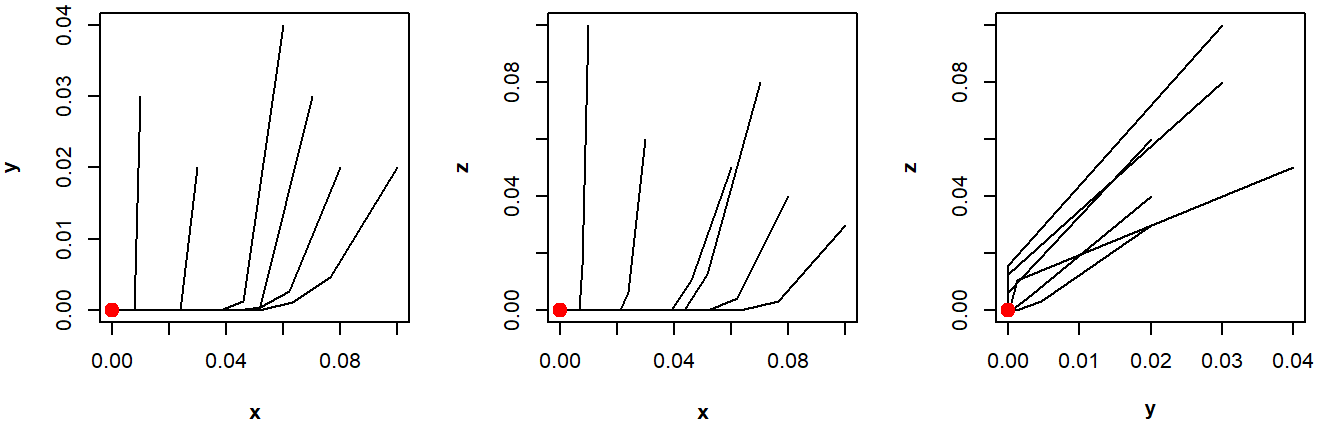
\includegraphics[width=1\linewidth]{images/Chapter 5/unnamed-chunk-3-1.png}     
   \caption{Example of orbits converging to $P_1$ \protect\footnotemark[1]}
\end{figure}

\footnotetext[1]{The fixed points will be color-coded as follows: $P_1$ in red, $P_2$ in orange, $P_3$ in green, and $P_4$ in blue.}

\section{Zone B}

In this zone $1<\mu<\frac{\beta}{\beta-1}<5/3$, so the system has two fixed points: the origin $P_1$ and $P_2 = (1 - \frac{1}{\mu}, 0, 0)$.
\\
$P_1$ is a saddle point, while $P_2$ is a locally asymptotically stable sink node. 
This implies that in this zone, only the prey population will survive.

It is important to note that the behaviour of the prey population $x$ is governed by the logistic map $\lambda_\mu(x) \coloneqq \mu x(1-x)$, this means that $x_n \leq \lambda_\mu(x_{n-1})$. Additionally, if $\mu\leq 2$ (as in our case), then $0\leq x_n \leq \lambda_\mu(x_0) \leq \frac{1}{2}, \, \forall \, n\in\N$. This implies that the prey population will be able to invade at most half of the carrying capacity.

It is also worth mentioning that the fixed point of the logistic map $\lambda_\mu(x)$ is asymptotically stable.

Therefore, given these premises, we can state that in this zone, starting from $(x_0, y_0, z_0)\in S$, three possible phenomena can happen:
\begin{itemize}
    \item $\exists \,  n\geq 0$ s.t. $x_n=0$. In this case $T(x_n,y_n,z_n)=(0,0,0) =  P_1$. This may happen, for example, when the carrying capacity $K=1$ is surpassed. In terms of the mathematical model, this occurs when $1-x-y-z\leq 0$, which we interpret simply as $1-x-y-z=0$. In biological terms, this means that the hunting of the predator species and the pressure of the top predator species on the prey species will lead to the extinction of the latter in one single iteration (due to the discrete nature of the model).  
    
    \item $x_n \neq 0, \, \forall \, n\geq0$, but $\exists \,  n\geq 0$ s.t. $y_n=0$. In this case $T(x_n,y_n,z_n)=(x_{n+1},0,0) = (\lambda_\mu(x_n),0,0)$, which is the univariate logistic map. The system will converge to the only asymptotically stable fixed point $P_2=(1 - \frac{1}{\mu},0,0)$. 

    \item $x_n,y_n \neq 0, \, \forall \, n\geq0$.In this case the orbit will converge to the second fixed point $P_2$ under the action of T, meaning that:
$$\lim_{n\to\infty} T^n(x,y,z) = (1 - \frac{1}{\mu},0,0) = P_2$$
\end{itemize}

\begin{figure}[!h]
\centering
 \textbf{\footnotesize{$\mu>1$}}   
    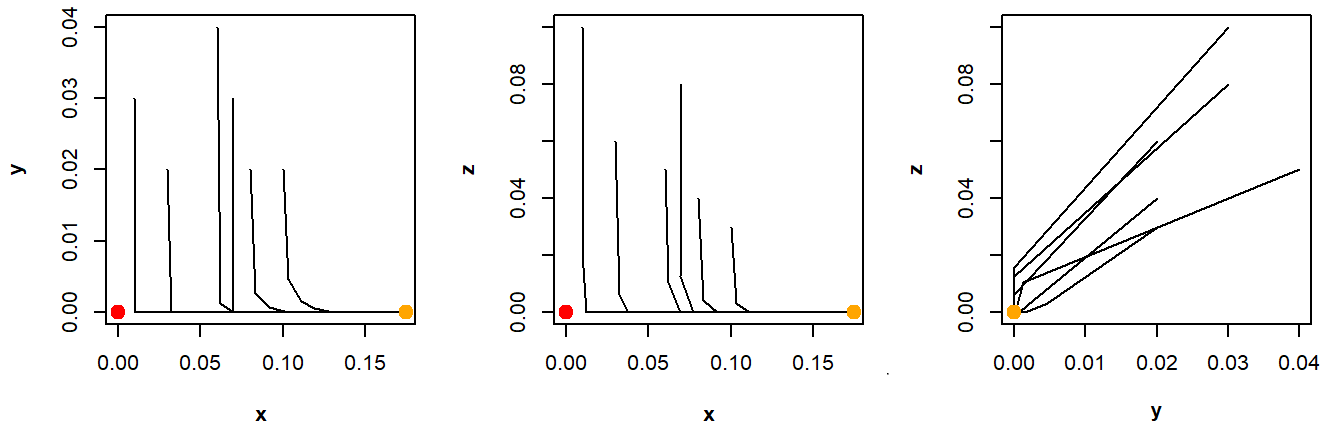
\includegraphics[width=1\linewidth]{images/Chapter 5/unnamed-chunk-5-1.png} 
    \caption{Example of orbits converging to $P_2$}
\end{figure}


\chapter{Chaotic behavior} 

As seen in section 4, the lack of stable fixed points in Zone F suggests the existence of chaotic attractors.
In order to formally identify chaos, the Lyapunov exponents should be computed, using a computational method. These exponents have allowed for the identification of points where bifurcations take place. It is also worth noting that the Lyapunov exponent is positive in chaotic systems.

\section{Influence of $\gamma$}
In this section, we investigate the impact of the parameter $\gamma$ on the behaviour of the system by fixing $\mu = 2.1$ and $\beta = 3.36$. Specifically, we examine how the increase in $\gamma$, while keeping $\mu$ and $\beta$ constant, leads to a transition from Zone E to Zone F. This transition is marked by a Neimark-Sacker bifurcation.

We remind that a Neimark-Sacker bifurcation is characterized by the emergence of a closed invariant curve. In the context of this system, this bifurcation occurs when the maximal Lyapunov exponent becomes zero, and the fixed point $P_4$ undergoes a change in stability, transitioning from stable to unstable, through a pair of complex eigenvalues with unit modulus. It is also worth mentioning that the bifurcation, in this case is supercritical, meaning that the resulting closed invariant curve is stable.
%http://www.scholarpedia.org/article/Neimark-Sacker_bifurcation

\begin{wrapfigure}{r}{0.3\textwidth}
\begin{center}
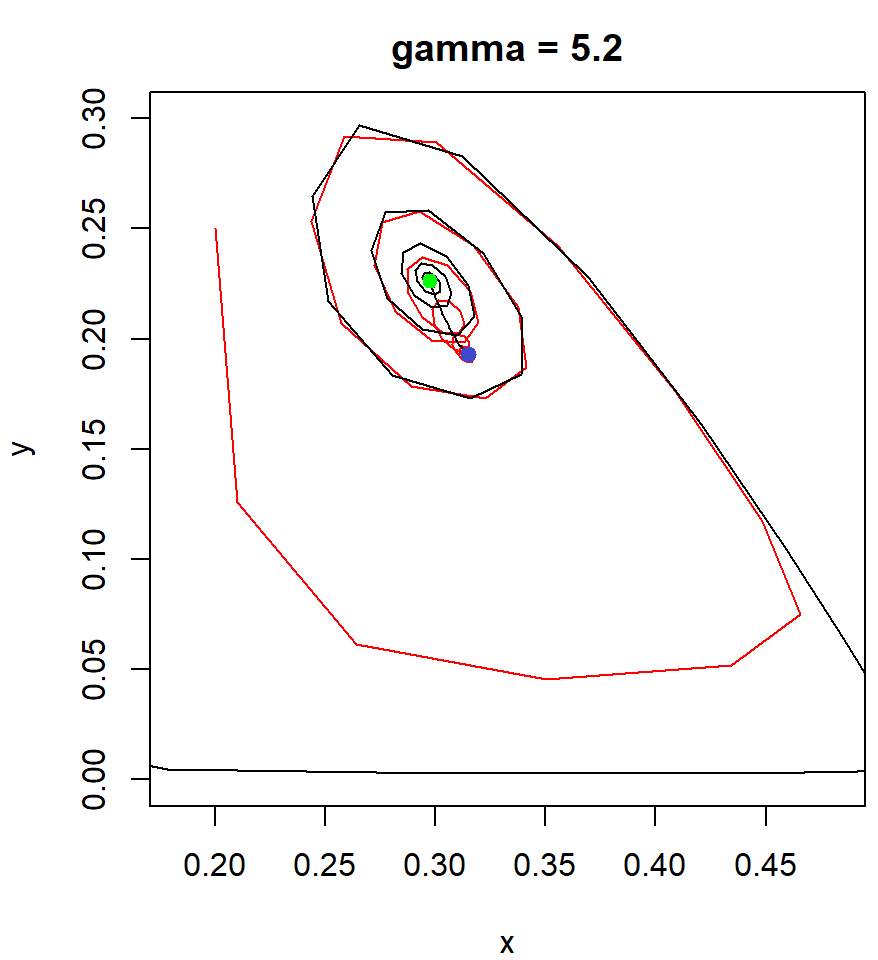
\includegraphics[width=0.29\textwidth]{images/Chapter 6.1/unnamed-chunk-2-1.png}
\end{center}
\caption{\footnotesize{Convergent orbit}}
\label{fig:Converging}
\end{wrapfigure}

Let's look at the situation in detail:
\begin{itemize}
\item For $5 < \gamma < 5.673555$ (i.e. Zone E) we have $P_4$ as the unique stable fixed point and all the orbits converge to this point. This static equilibrium, in which the three species coexist, is reached after damped oscillations, as illustrated in \autoref{fig:Converging}.
\item For $5.673555 < \gamma < 7.25$ (i.e. Zone F) all fixed points become unstable, resulting in the presence of chaotic and periodic solutions. In this range of values, we can observe closed invariant curves, whose periods increase as $\gamma$ increases (\autoref{fig:invariant_curves}).
\item For $7.25 < \gamma < 9.4$  we identify a route to chaos driven by a sequence of period-doubling invariant closed curves (\autoref{fig:chaotic_behav}).
\end{itemize}

\begin{figure}[H]
\minipage{0.32\textwidth}
  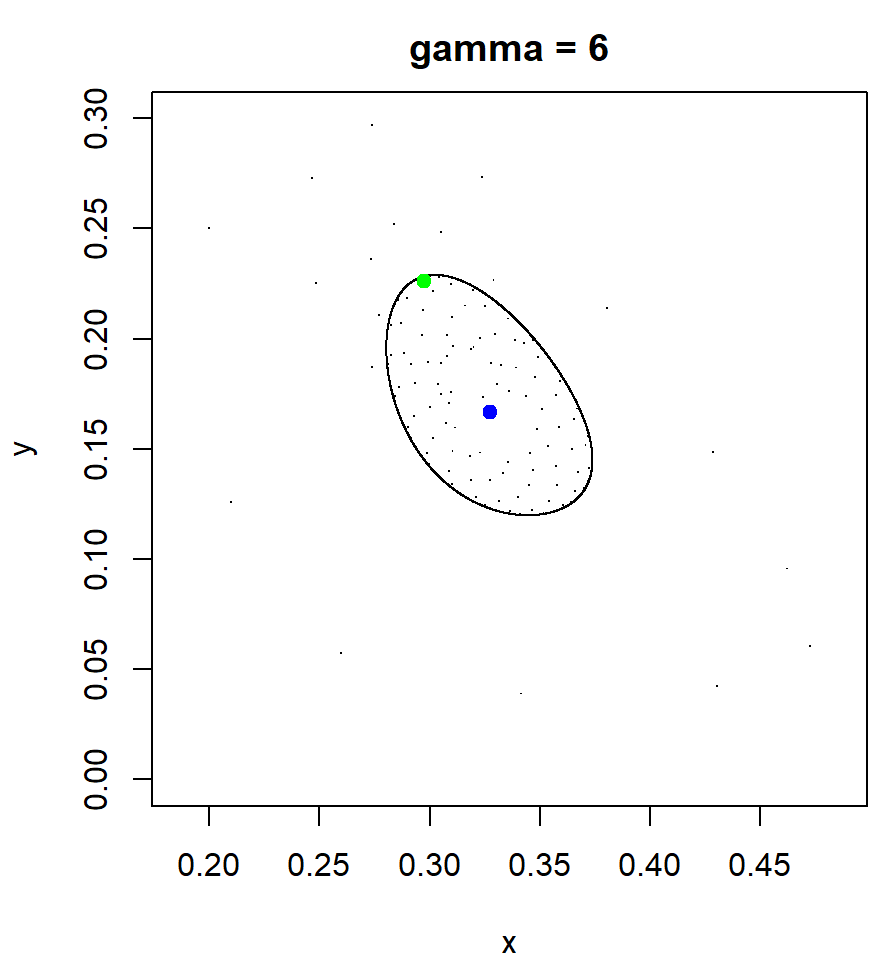
\includegraphics[width=\linewidth]{images/Chapter 6.1/unnamed-chunk-3-1.png}
\endminipage\hfill
\minipage{0.32\textwidth}
  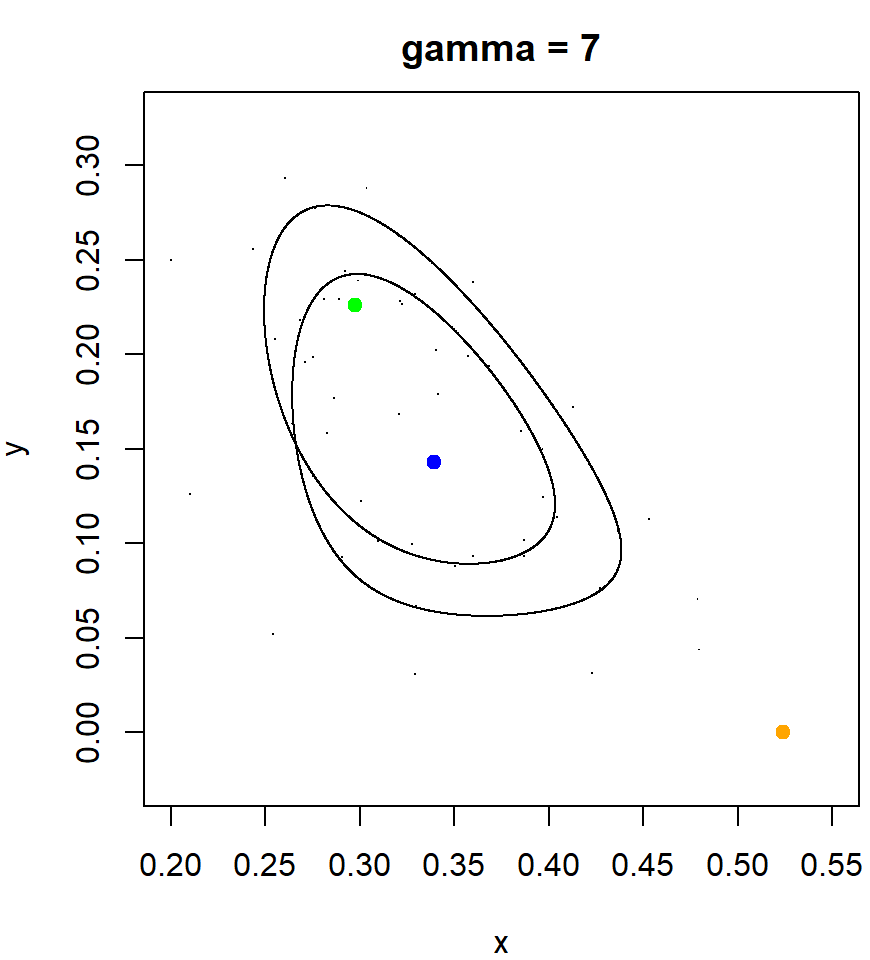
\includegraphics[width=\linewidth]{images/Chapter 6.1/unnamed-chunk-4-1.png}
\endminipage\hfill
\minipage{0.32\textwidth}
  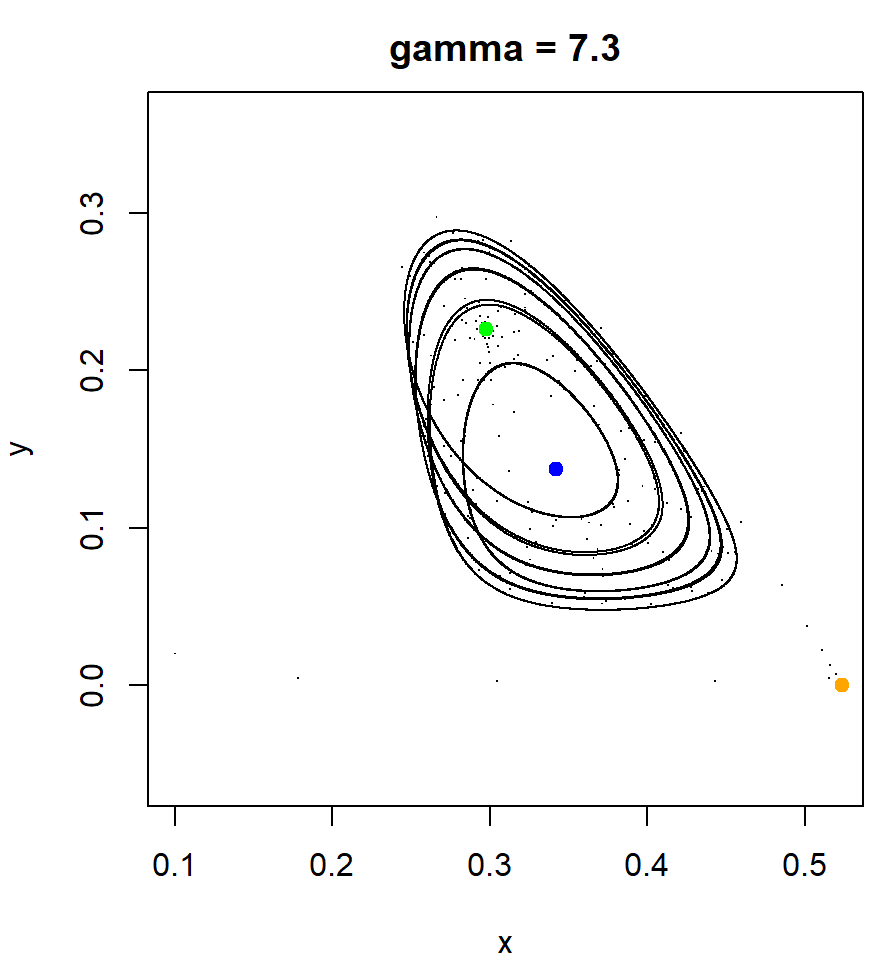
\includegraphics[width=\linewidth]{images/Chapter 6.1/unnamed-chunk-6-1.png}
\endminipage
\caption{Closed invariant curves of different periods}
\label{fig:invariant_curves}
\end{figure}

In essence, an increase in the predation rate of species z destabilizes the dynamics of the system, leading to chaotic fluctuations among the three species.

\begin{figure}[H]
\minipage{0.32\textwidth}
  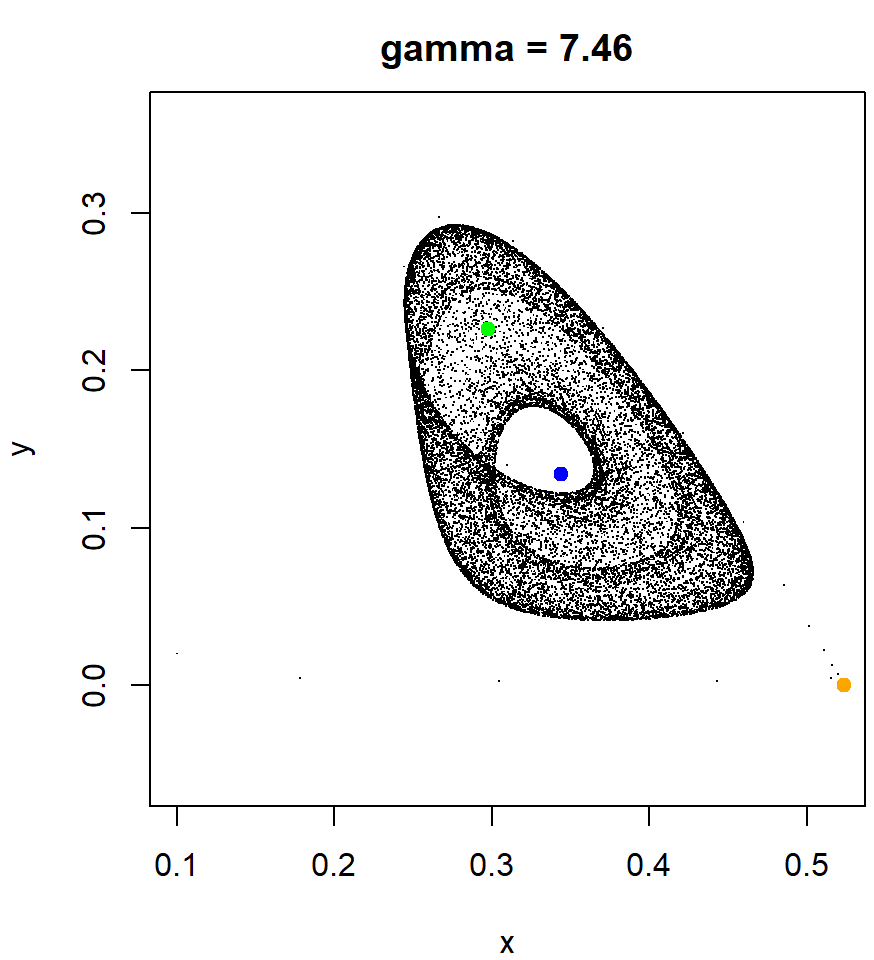
\includegraphics[width=\linewidth]{images/Chapter 6.1/unnamed-chunk-8-1.png}
\endminipage\hfill
\minipage{0.32\textwidth}
  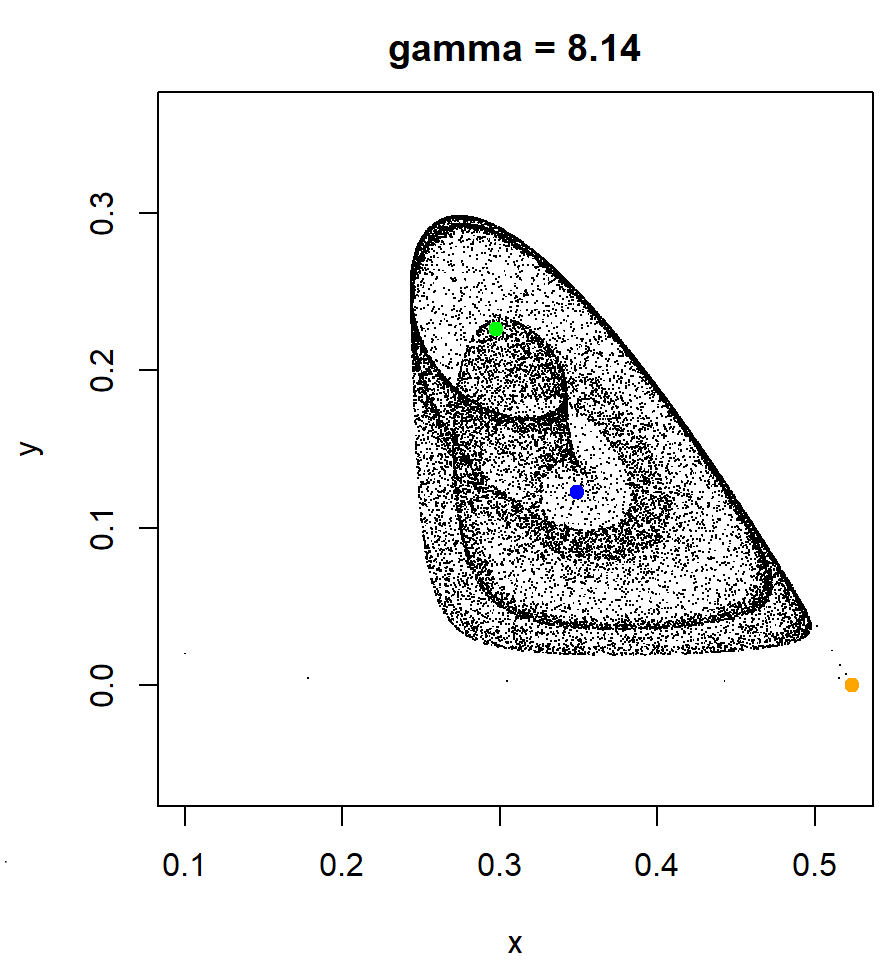
\includegraphics[width=\linewidth]{images/Chapter 6.1/unnamed-chunk-10-1.png}
\endminipage\hfill
\minipage{0.32\textwidth}%
  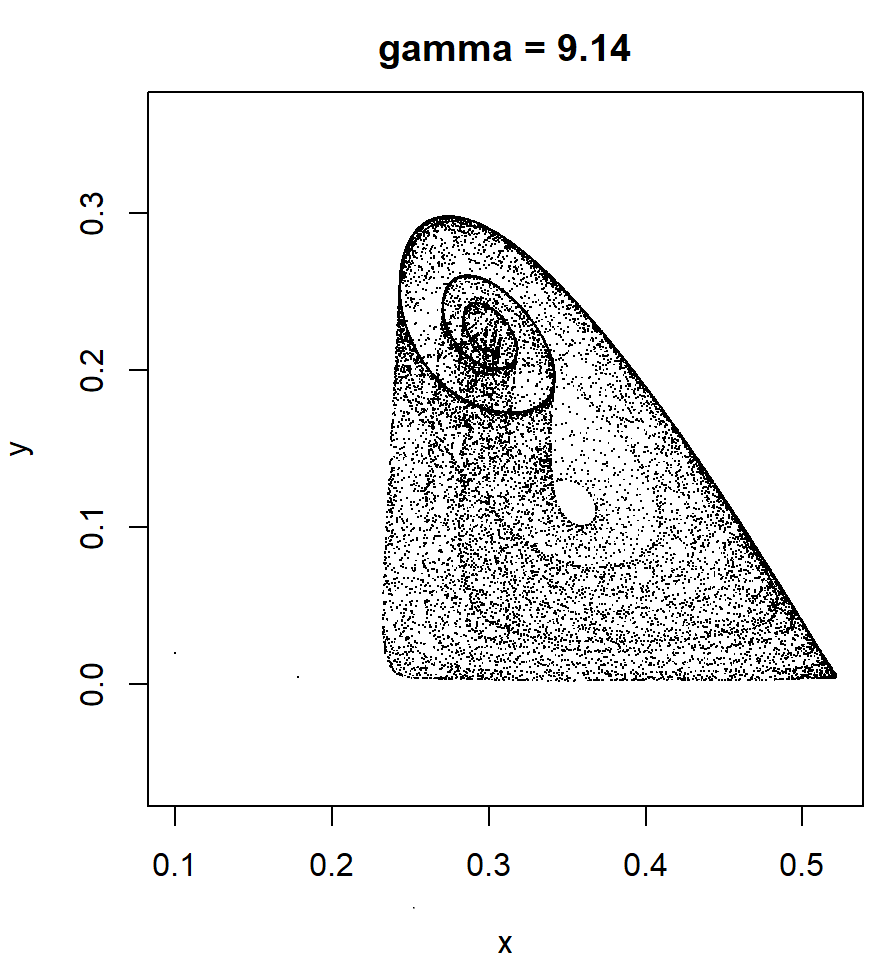
\includegraphics[width=\linewidth]{images/Chapter 6.1/unnamed-chunk-12-1.png}
\endminipage
\caption{Degeneration to chaotic behaviour}
\label{fig:chaotic_behav}
\end{figure}

\begin{figure}[H]
\centering
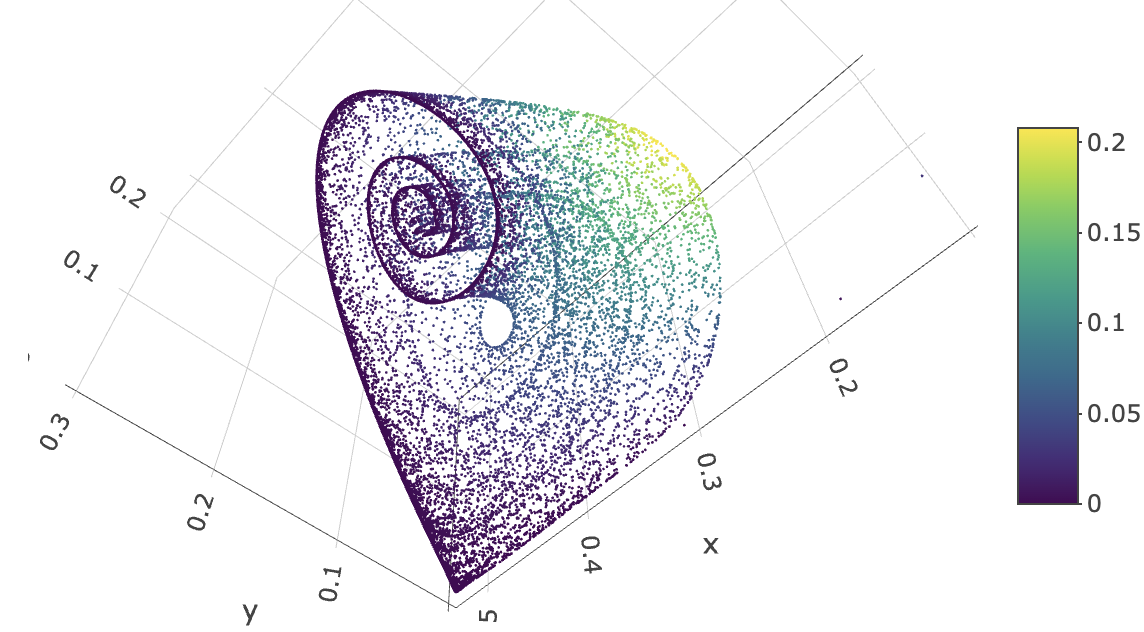
\includegraphics[width=0.8\linewidth]{3dcolor.png}
\caption{3-dimensional diagram of chaotic orbits ($\gamma=9.14$)}
\end{figure}

\section{Influence of $\beta$}

We consider $\beta$ in the range $[2.5, 5]$:

\begin{itemize}
    \item for $2.5\leq \beta \leq 2.70297$ (i.e. zone D) the top predator $z$ goes to extinction and the prey and predator $y$ achieve a static
equilibrium
    \item for $2.70297 \leq \beta \leq 3.1804935$ (i.e. zone E) $P_3$ becomes unstable and $P_4$ becomes stable. Counter-intuitively, stronger predation of $y$ on $x$ makes the three species coexist, avoiding the extinction of the top predator $z$.

    \item for $3.1804935 \leq \beta \leq 3.\overline{81}$ (i.e Zone F) all of the fixed points are unstable and thus periodic dynamics can occur.

    \item for $3.\overline{81} \leq \beta \leq5$ (i.e. Zone G) the same behaviour of the previous interval is expected, all the three species coexist, without stopping in an equilibrium point.
\end{itemize}

\begin{figure}[!htb]
\centering
    \begin{tabular}{ccc}
    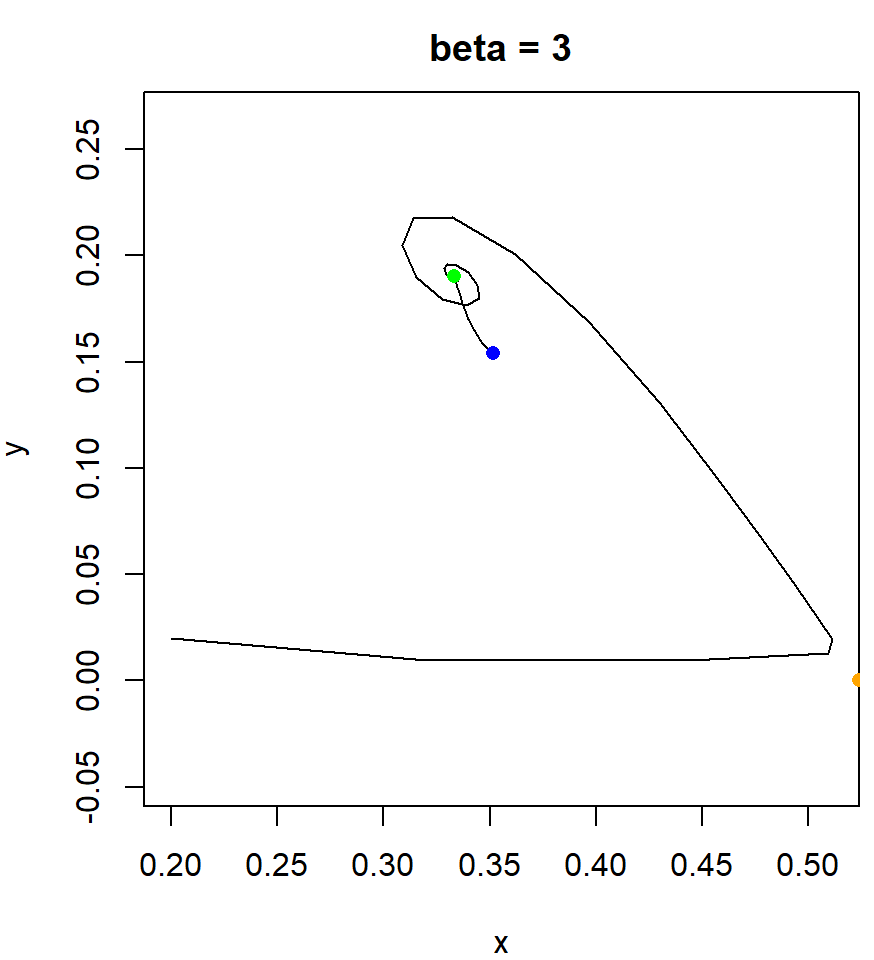
\includegraphics[width=0.32\linewidth]{images/Chapter 6.2/unnamed-chunk-5-1.png} &
    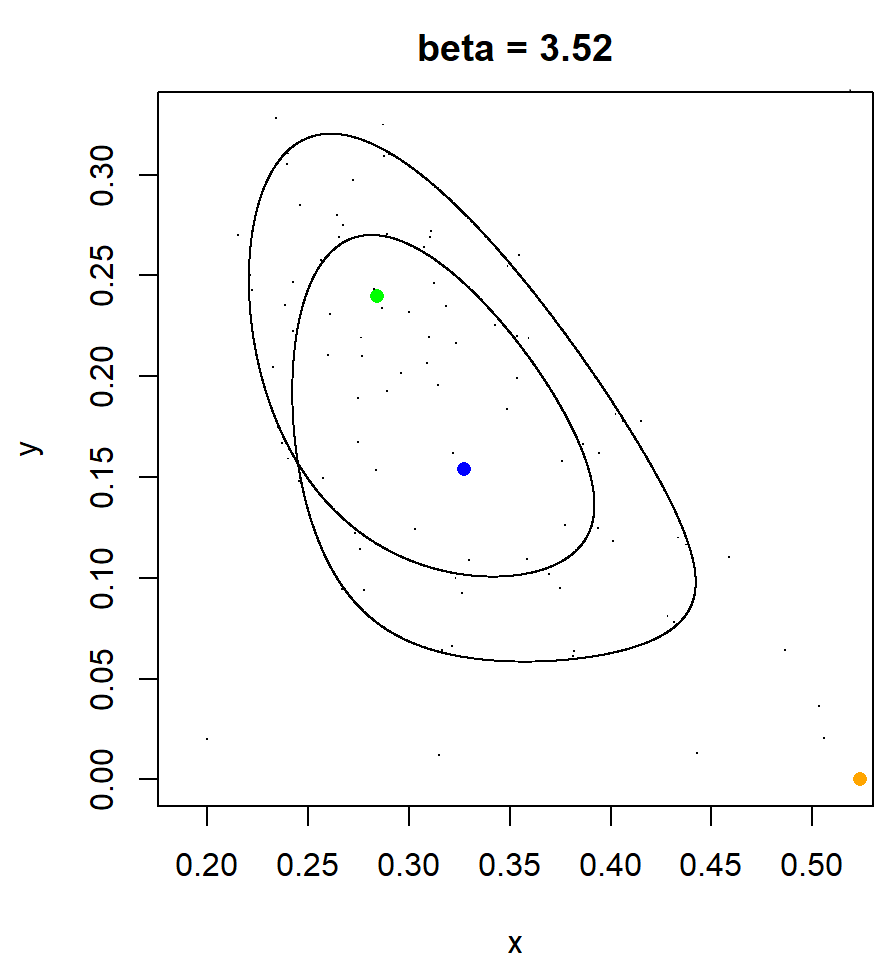
\includegraphics[width=0.32\linewidth]{images/Chapter 6.2/unnamed-chunk-7-1.png} &
    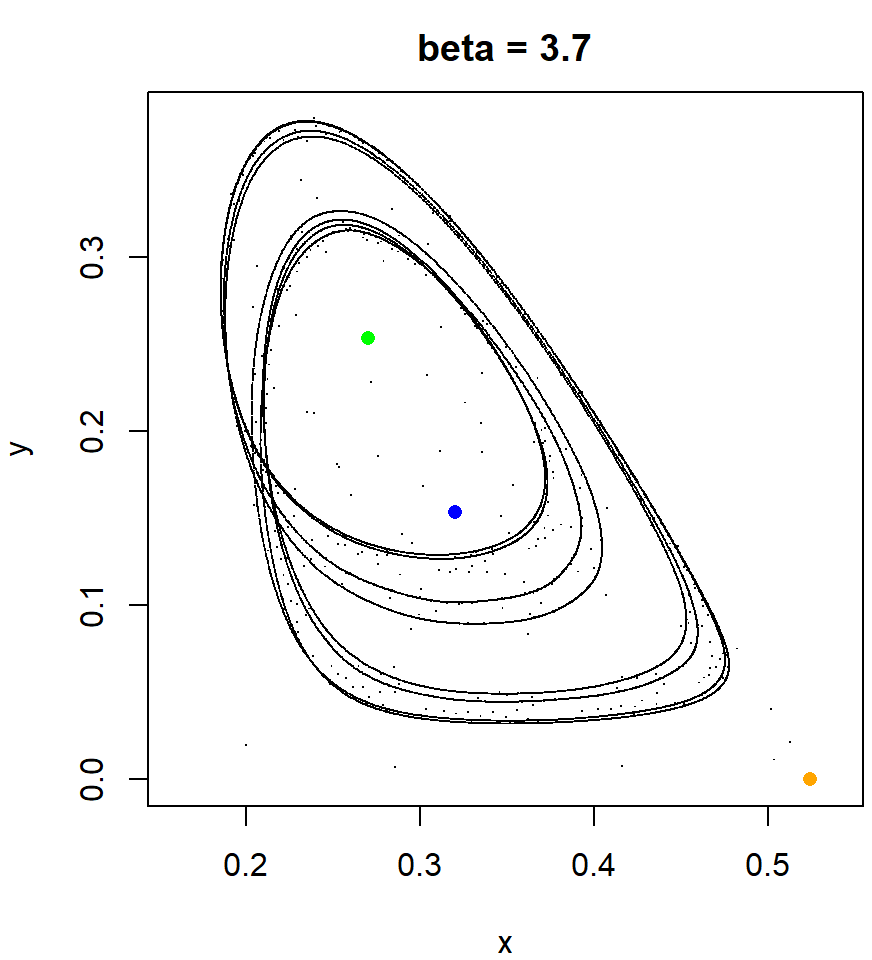
\includegraphics[width=0.32\linewidth]{images/Chapter 6.2/unnamed-chunk-8-1.png} &
    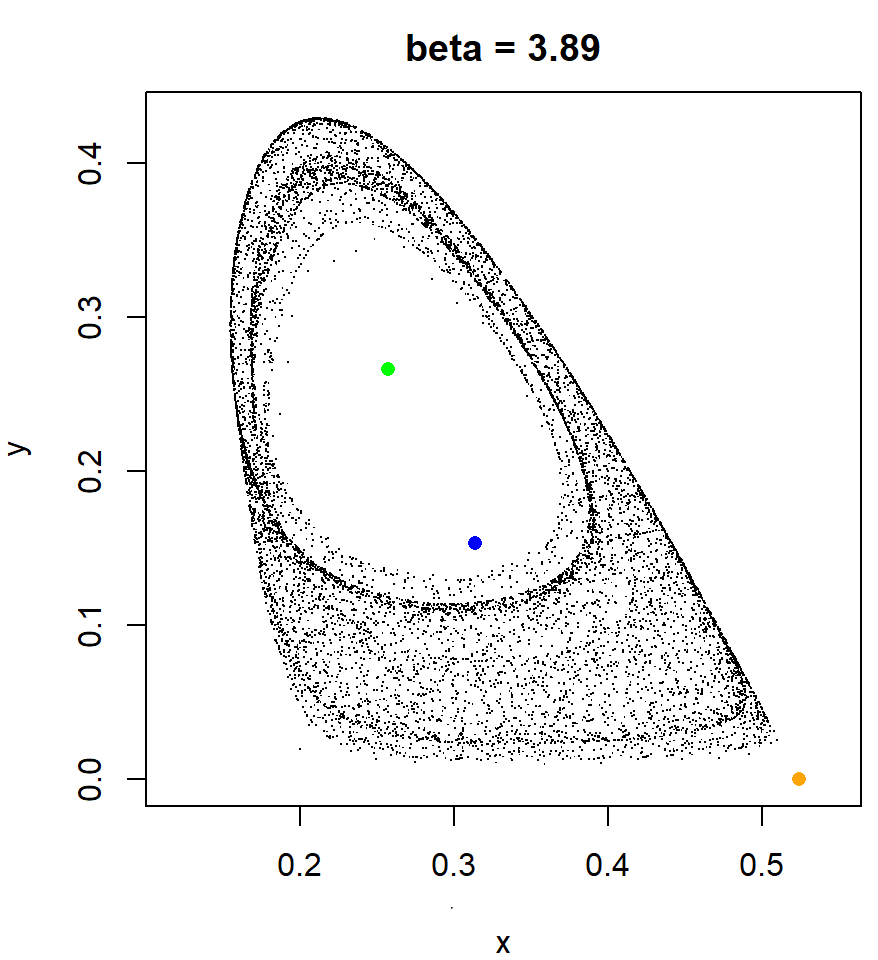
\includegraphics[width=0.32\linewidth]{images/Chapter 6.2/unnamed-chunk-9-1.png} &
    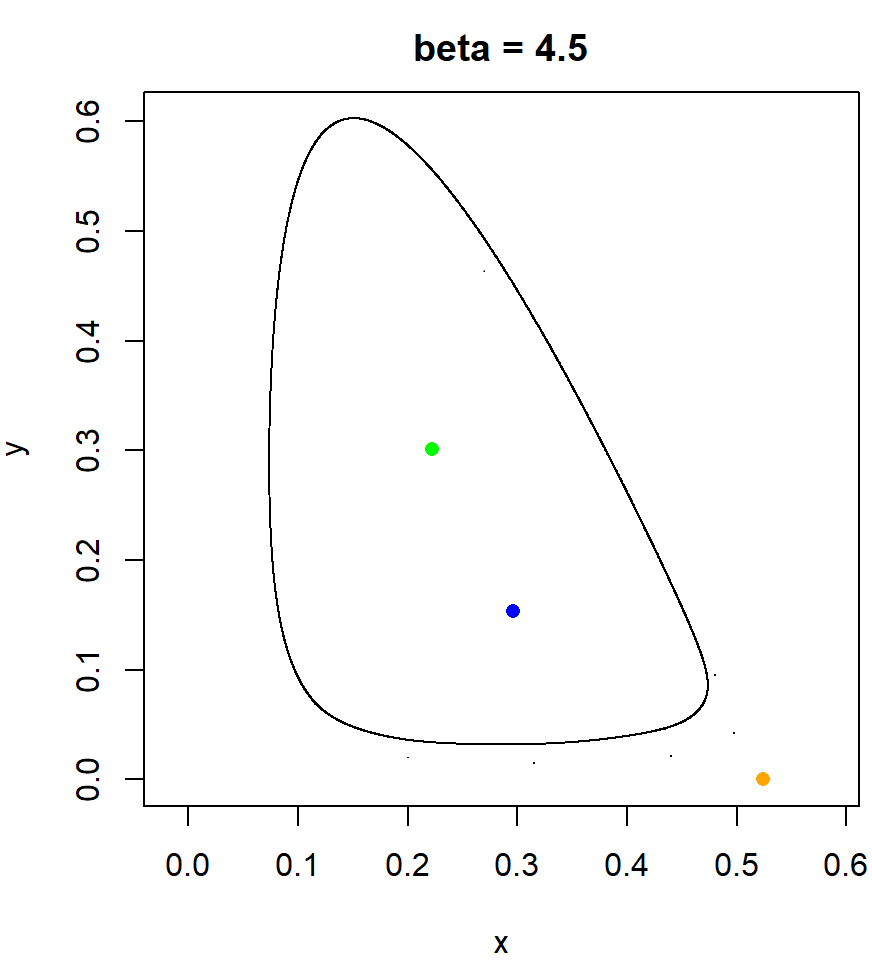
\includegraphics[width=0.32\linewidth]{images/Chapter 6.2/unnamed-chunk-10-1.png} &
    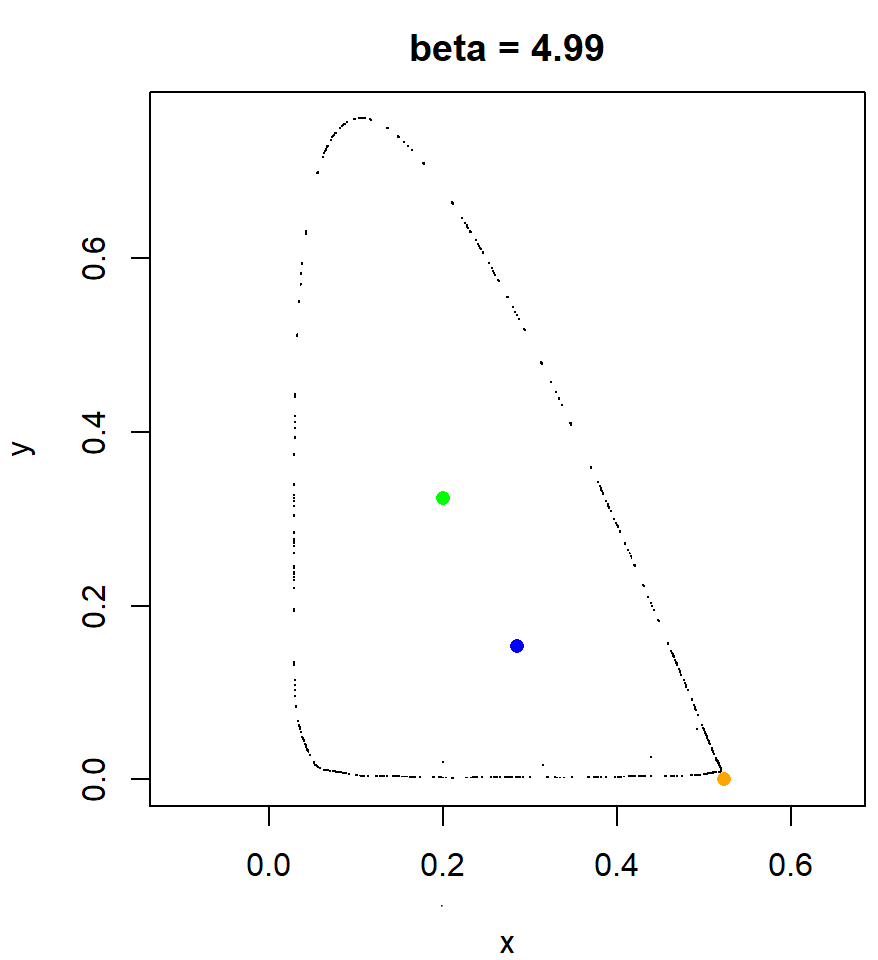
\includegraphics[width=0.32\linewidth]{images/Chapter 6.2/unnamed-chunk-12-1.png}
    \end{tabular}
  
   \caption{Transition from convergent behaviour to chaos}
\end{figure}

\section{Route to chaos}

Our analysis has revealed that our system enters into a chaotic regime through a period-doubling route, commonly known as the Feigenbaum scenario. This phenomenon occurs following a Neimark-Sacker bifurcation.

To more easily characterise the routes to chaos, we can let the predation parameters $\gamma$ and $\beta$ vary and plot the local maxima of the time series for $x_n$ for each value of these parameters. This will reveal period-$q$ invariant curves, which have $q$ distinct local maxima, with $q$ tending towards infinity in the chaotic region.

We can also exploit the Fast Fourier Transform (FFT) to determine the number of local maxima, which can be identified as the number of peaks in the magnitude of the Fourier coefficients. It should be noted that for a value of $\gamma=7.4$, a high number of peaks emerge, indicating a chaotic behaviour (\autoref{fig:Chaotic_fourier})

The local-maxima approach is particularly useful because by plotting them against the values of $\gamma$ and $\beta$ at which they appear, we can construct bifurcation diagrams that clearly display the classic branch-like structure of the period-doubling process  (\autoref{fig:Bif_diag_gamma} and \autoref{fig:Bif_diag_beta}).

\begin{figure}[!h]
\centering
\textbf{\footnotesize{$\gamma=6.8$}}
    \begin{tabular}{cc}
    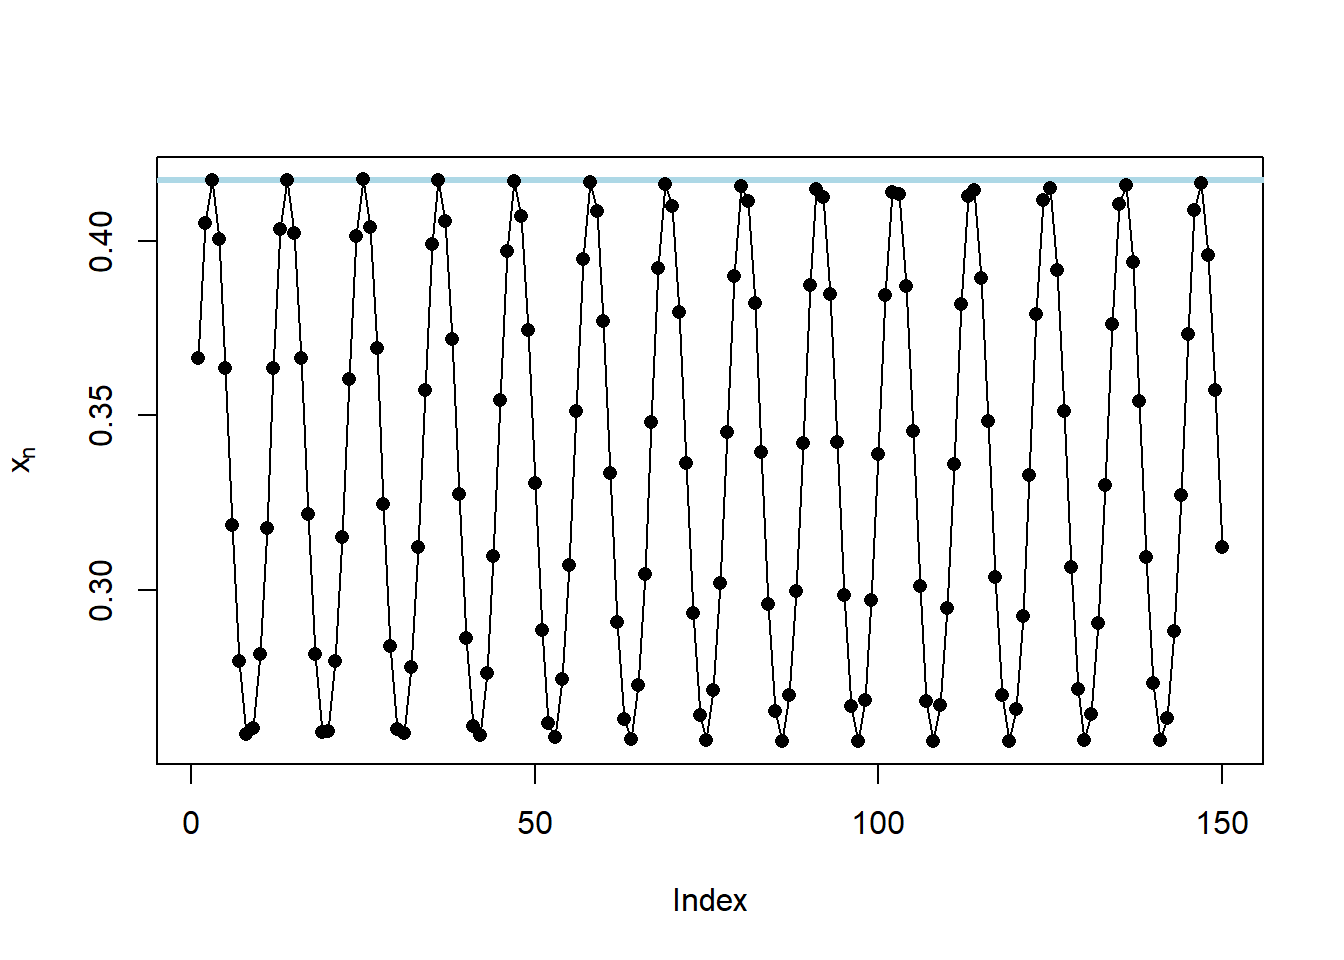
\includegraphics[width=0.45\linewidth]{images/Chapter 6.3/unnamed-chunk-3-1.png} &
    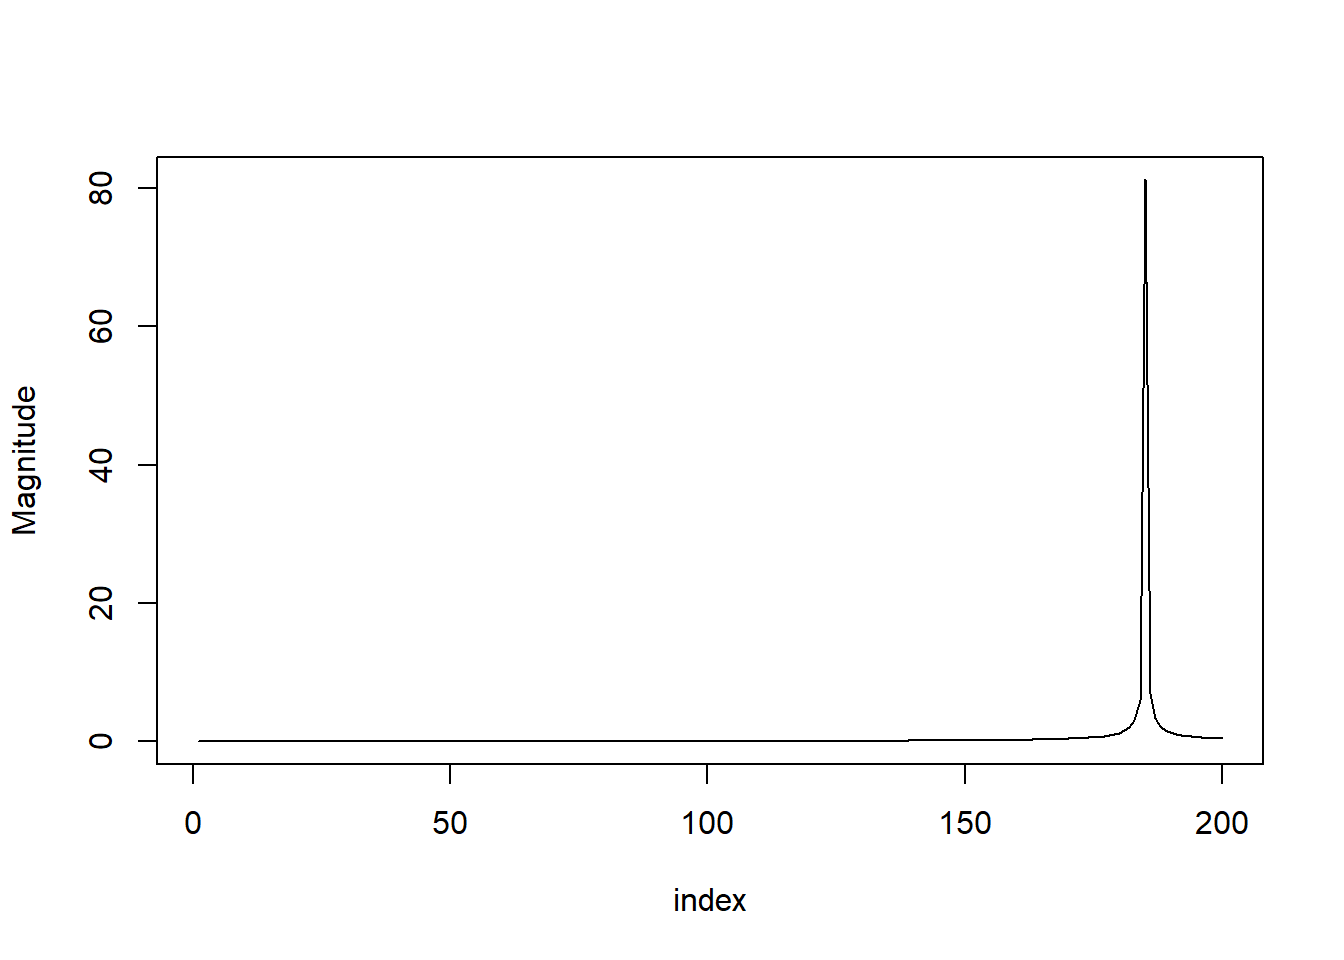
\includegraphics[width=0.45\linewidth]{images/Chapter 6.3/unnamed-chunk-4-1.png} 
    \end{tabular}
 \textbf{\footnotesize{$\gamma=7.1$}}   
    \begin{tabular}{cc}
    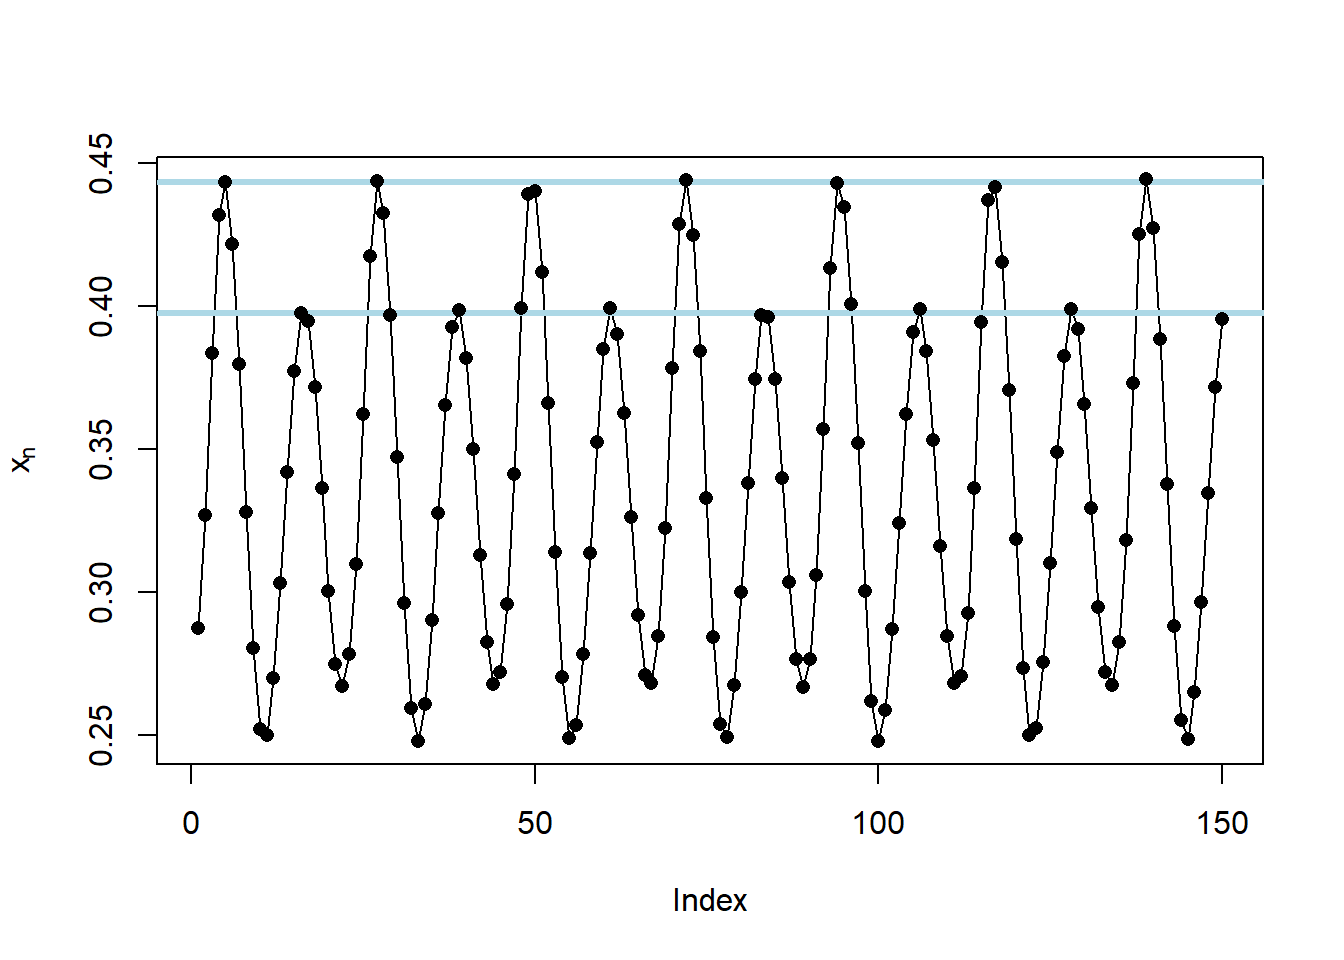
\includegraphics[width=0.45\linewidth]{images/Chapter 6.3/unnamed-chunk-5-1.png} &
    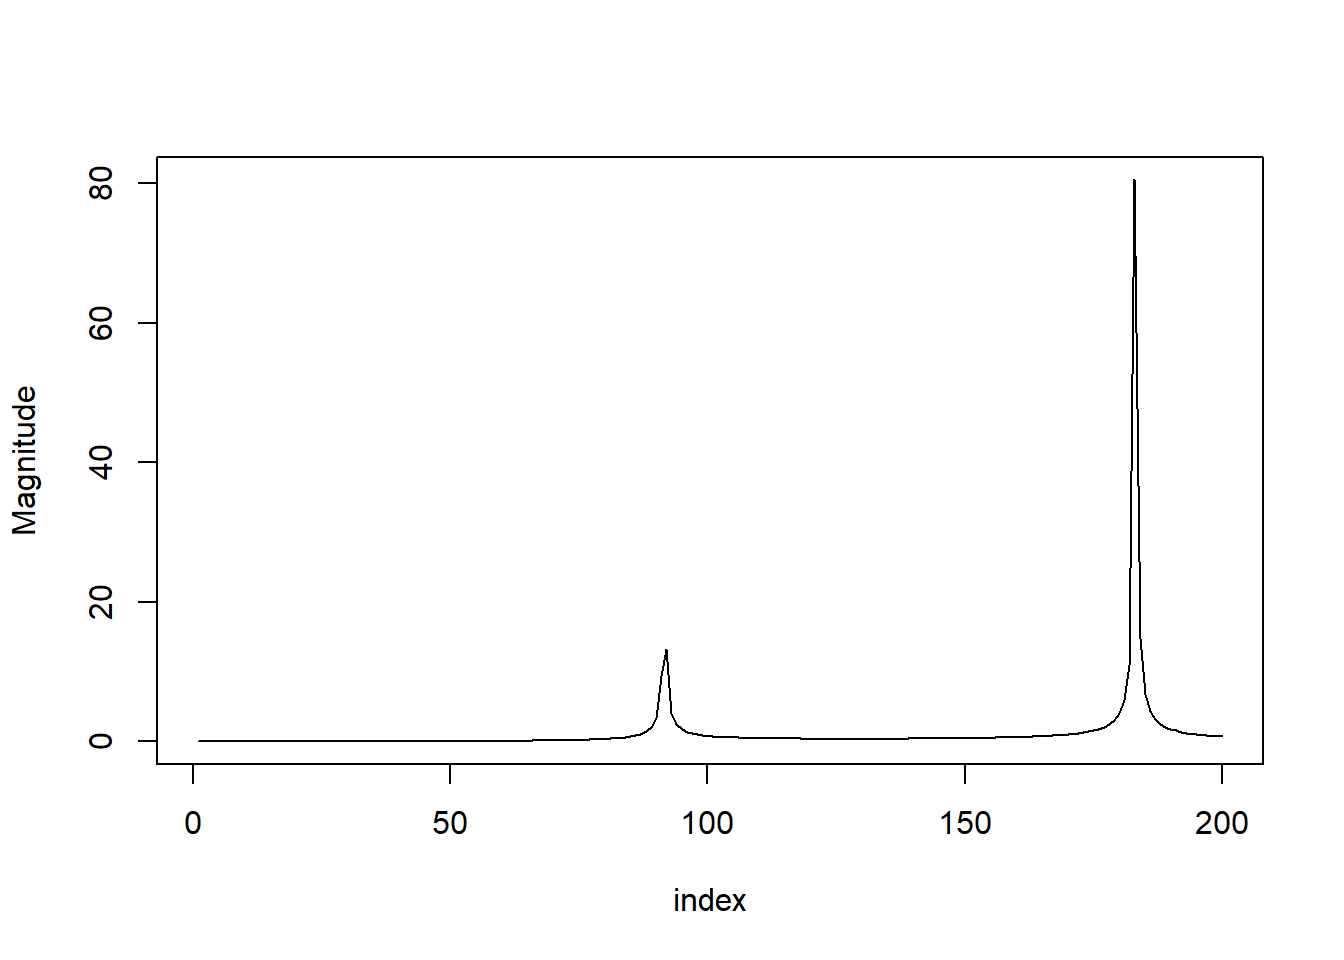
\includegraphics[width=0.45\linewidth]{images/Chapter 6.3/unnamed-chunk-6-1.png} 
    \end{tabular}
 \textbf{\footnotesize{$\gamma=7.18$}}   
    \begin{tabular}{cc}
    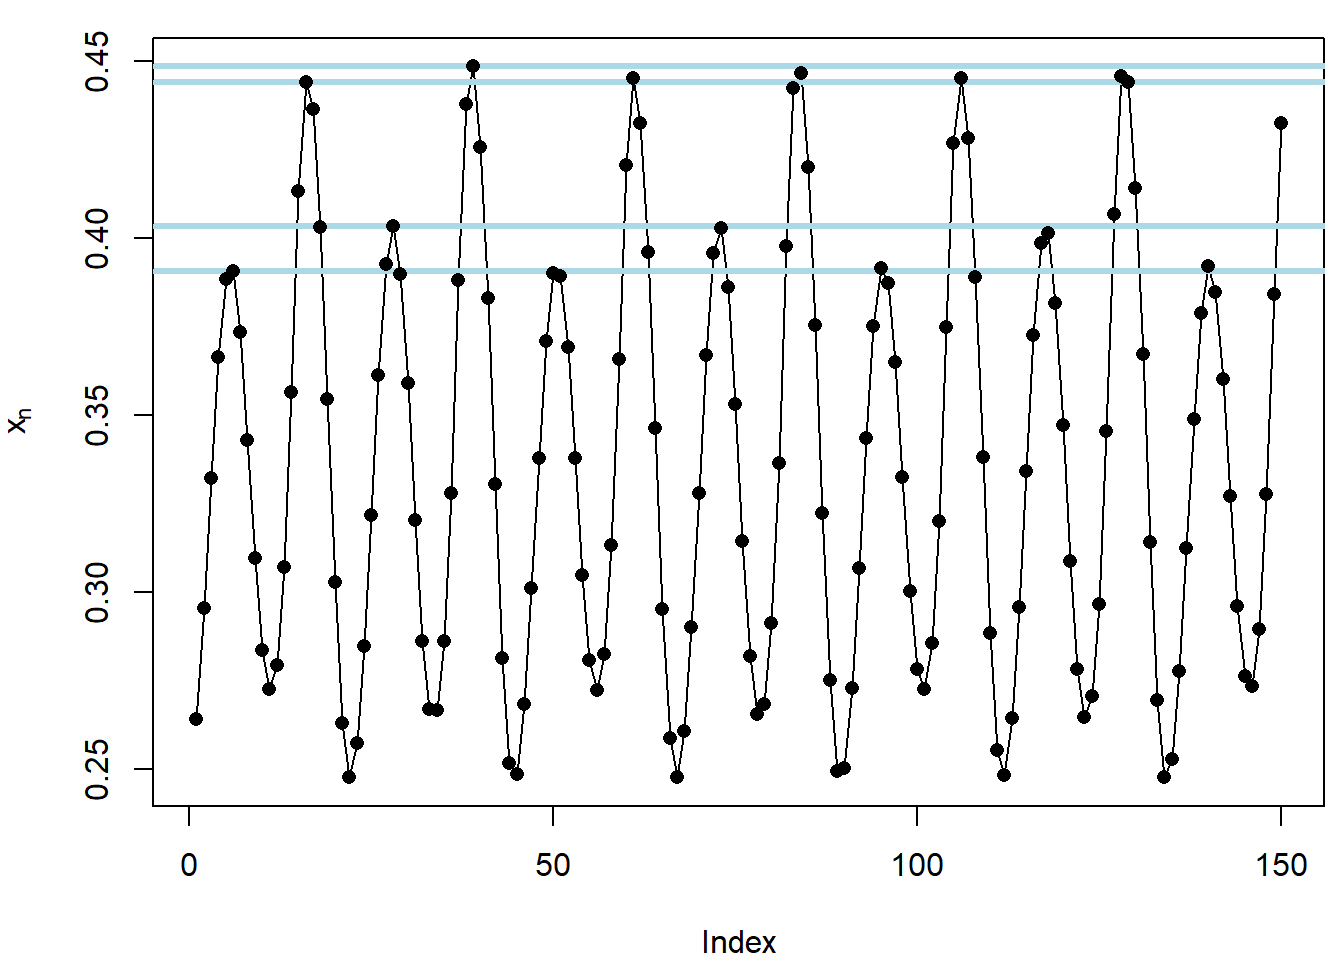
\includegraphics[width=0.45\linewidth]{images/Chapter 6.3/unnamed-chunk-7-1.png} &
    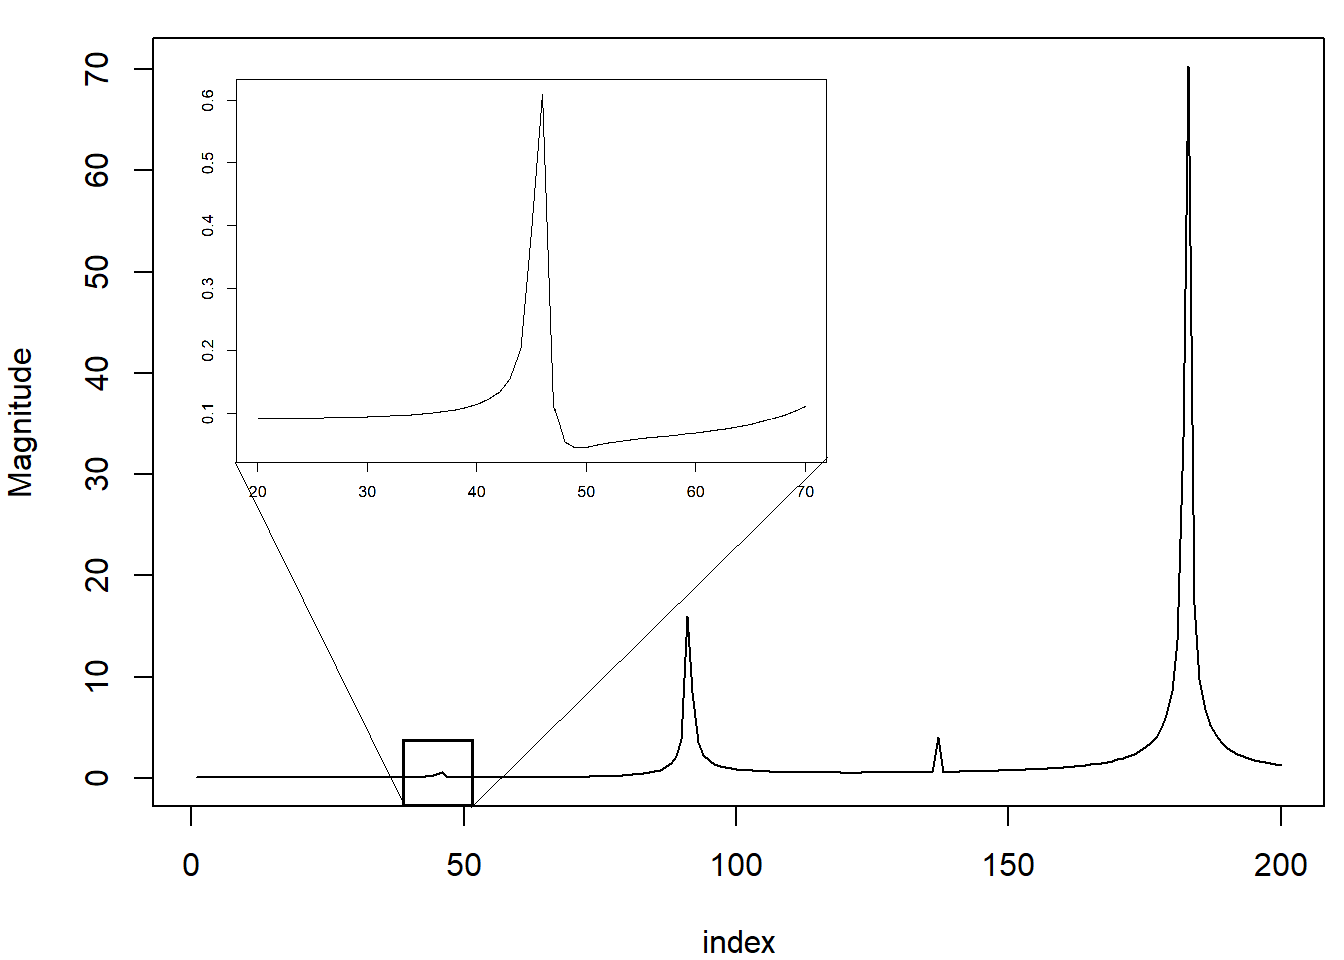
\includegraphics[width=0.45\linewidth]{images/Chapter 6.3/unnamed-chunk-8-1.png} 
    \end{tabular}
\end{figure}
\begin{figure}[!h]
\centering  
 \textbf{\footnotesize{$\gamma=7.4$}}   
    \begin{tabular}{cc}
    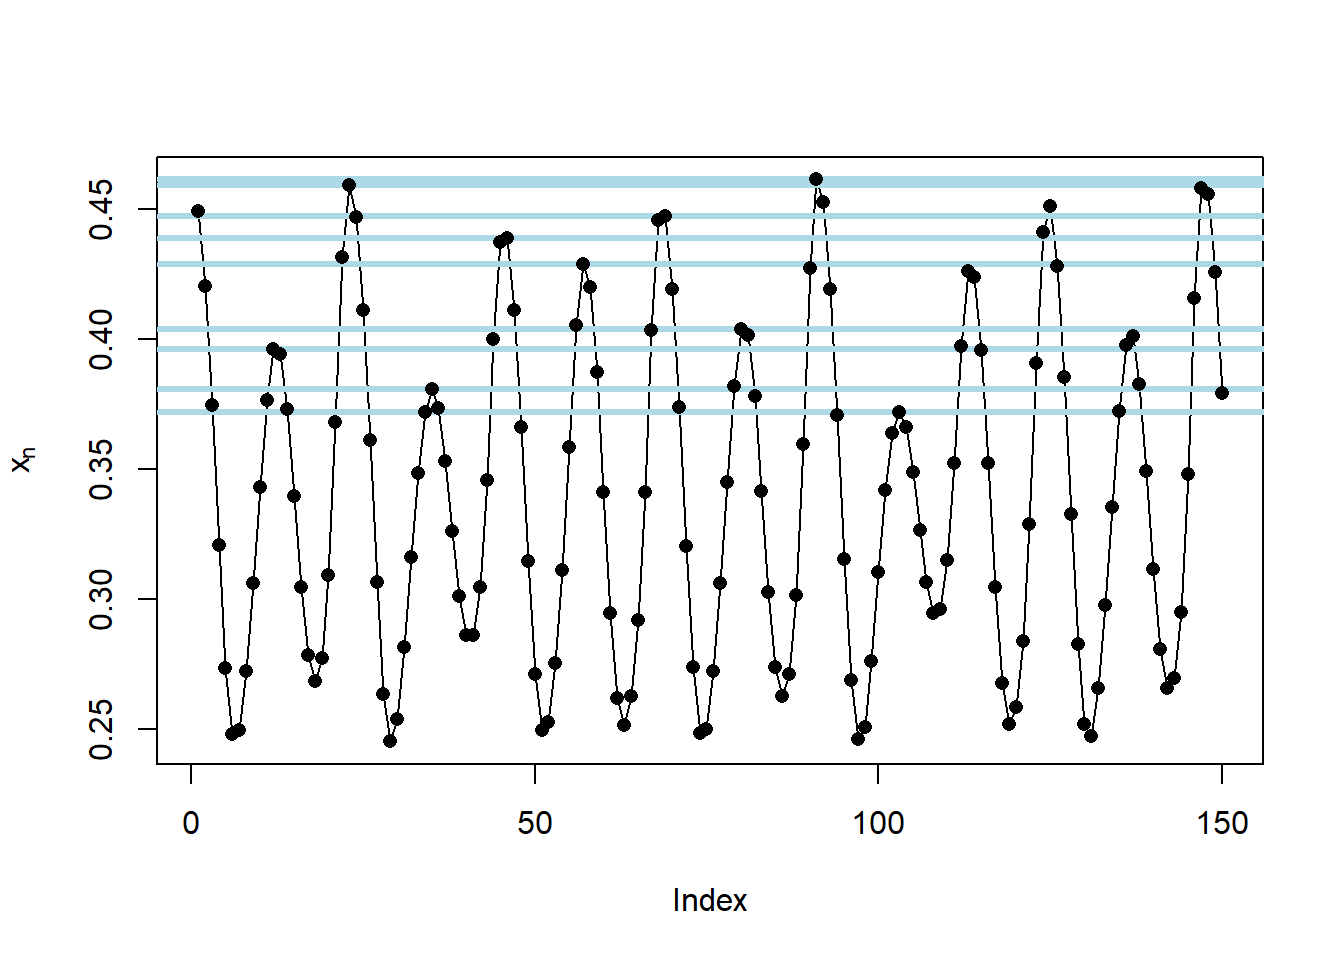
\includegraphics[width=0.45\linewidth]{images/Chapter 6.3/unnamed-chunk-9-1.png} &
    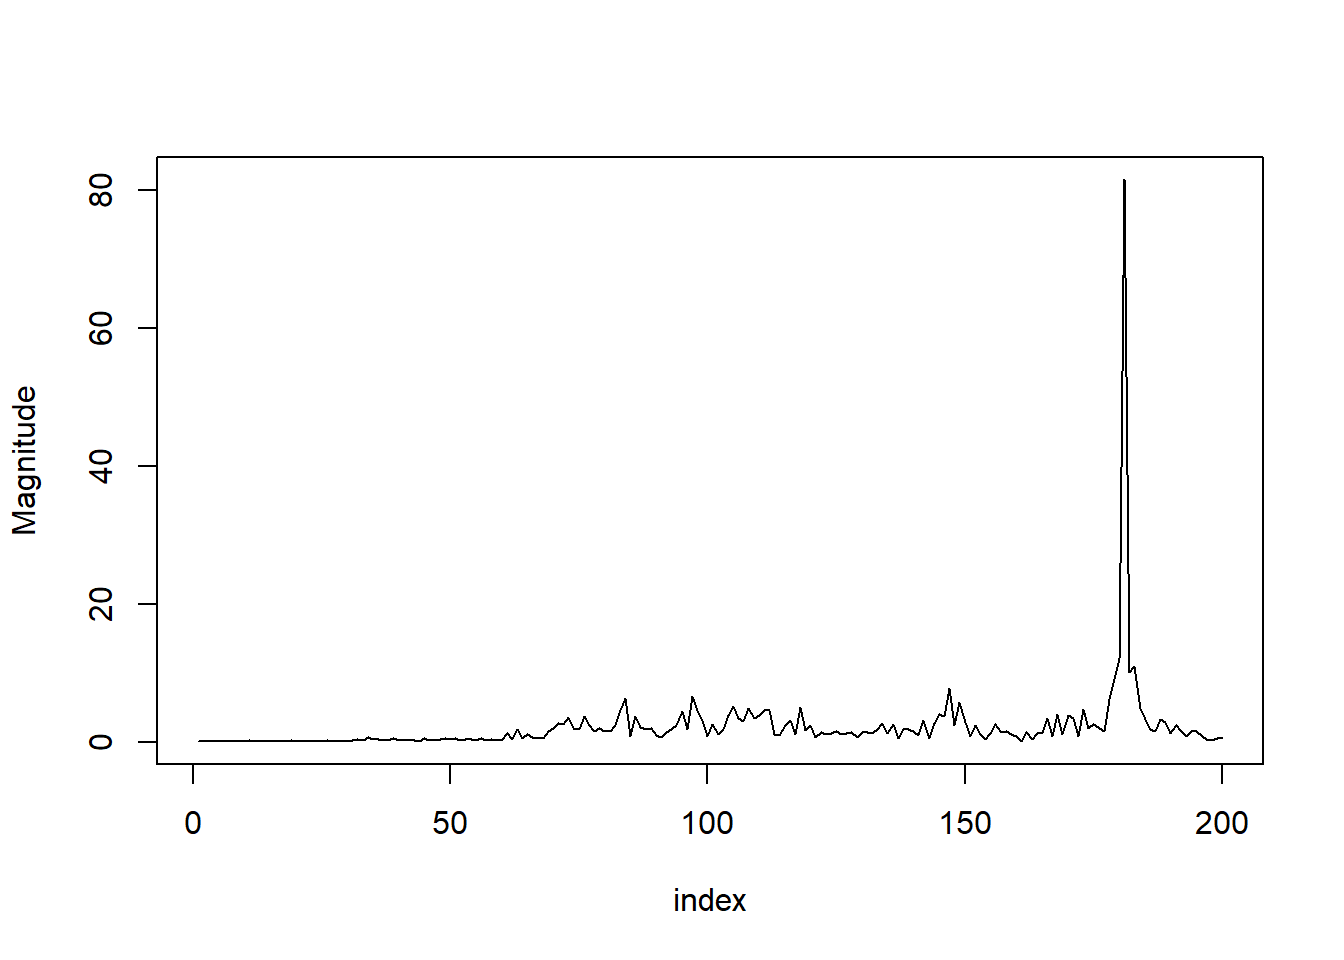
\includegraphics[width=0.45\linewidth]{images/Chapter 6.3/unnamed-chunk-10-1.png} &
    \end{tabular}
   \caption{Analysis of the local maxima of the closed invariant orbits}
   \label{fig:Chaotic_fourier}
\end{figure}

\begin{figure}[!h]
\centering
   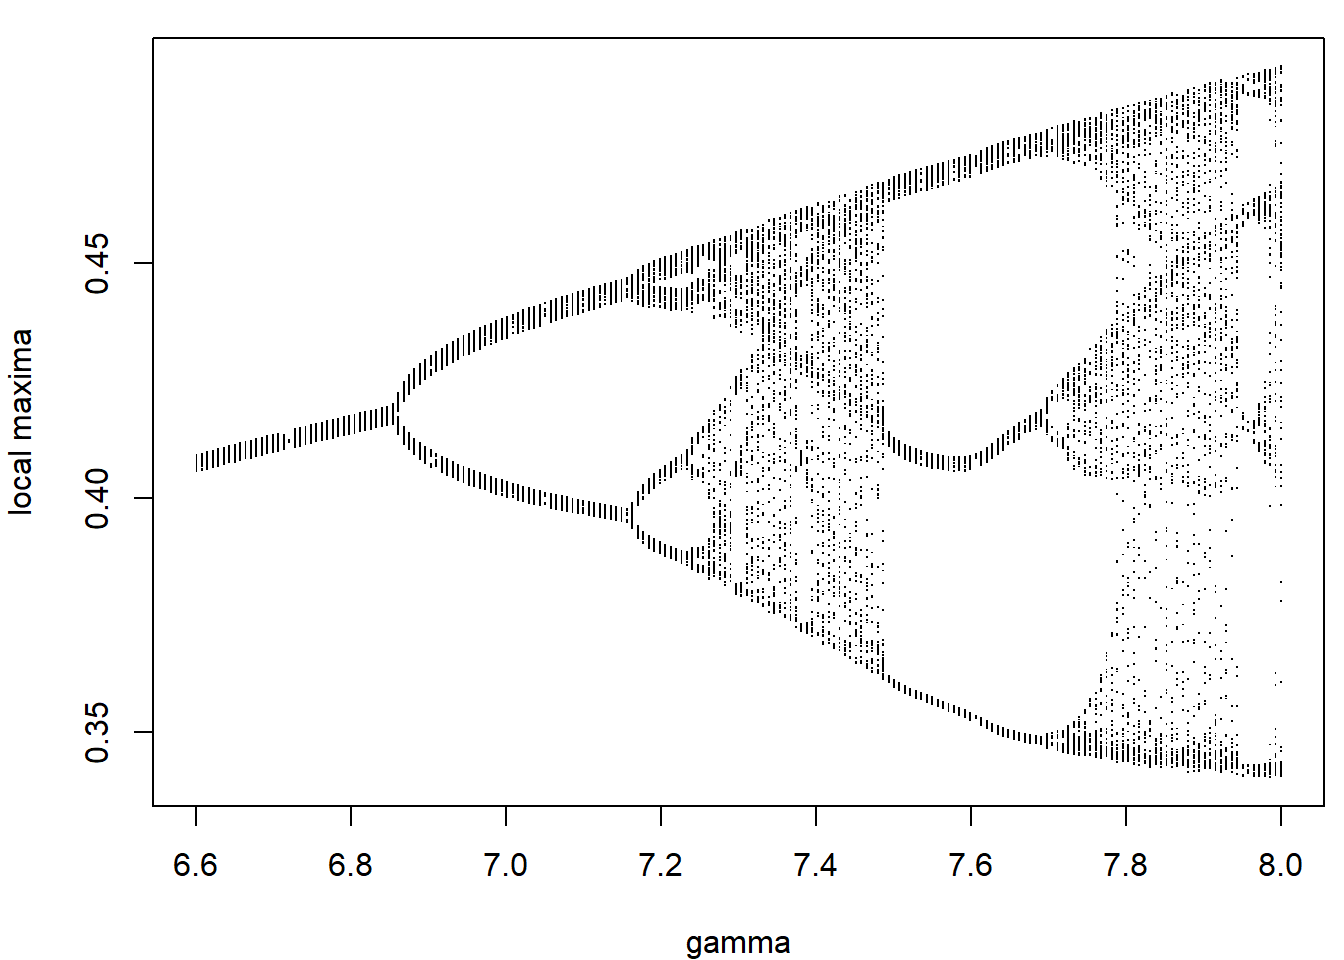
\includegraphics[width=0.6\linewidth]{images/Chapter 6.3/unnamed-chunk-11-1.png} 
  \caption{Diagrams displaying period-doubling of invariant curves w.r.t. $\gamma$}
  \label{fig:Bif_diag_gamma}
\end{figure}

\begin{figure}[!h]
\centering
   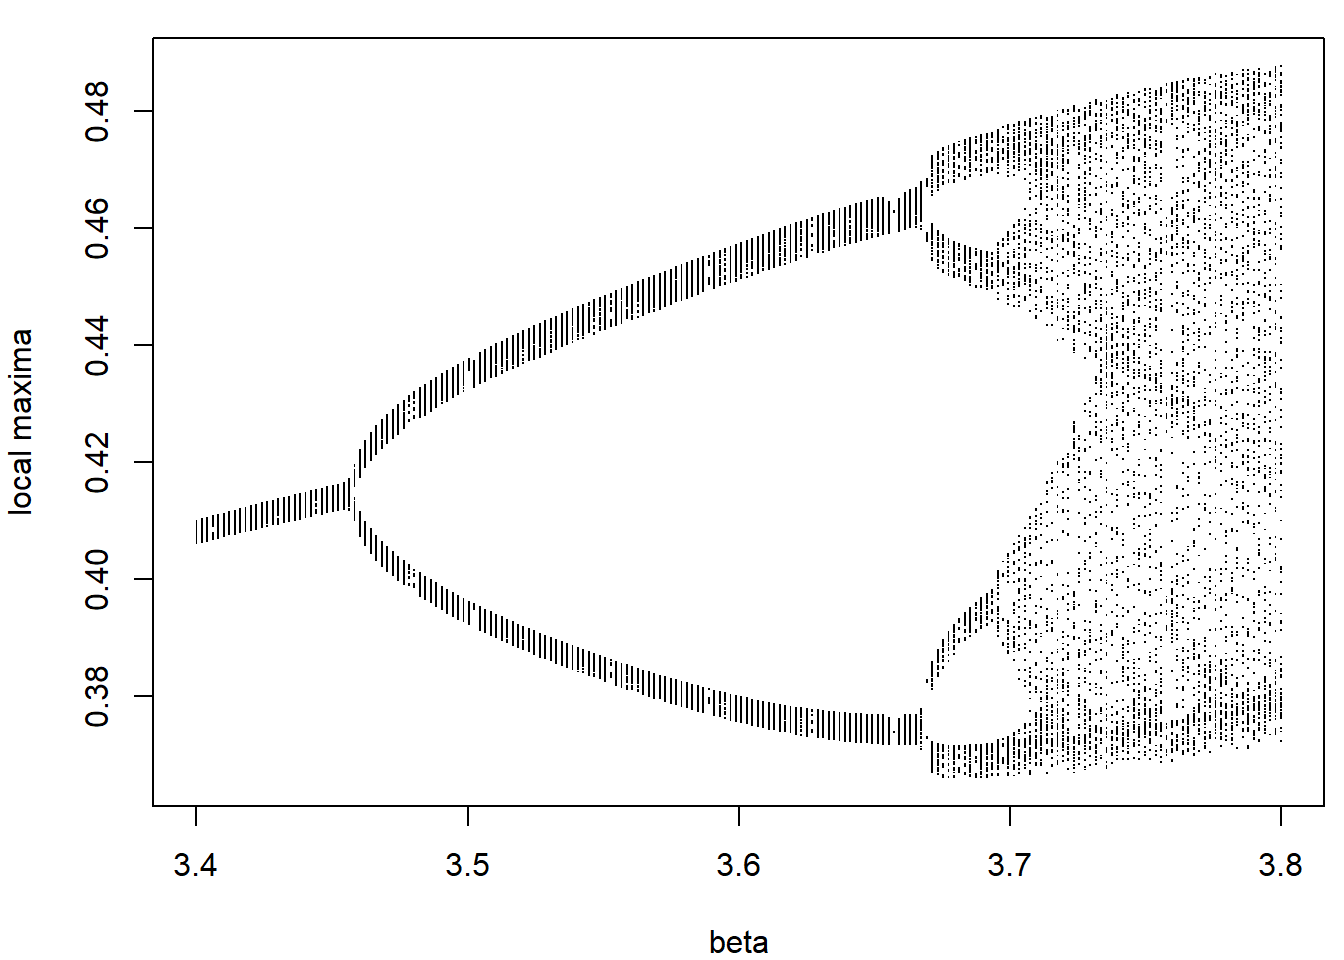
\includegraphics[width=0.6\linewidth]{images/Chapter 6.3/unnamed-chunk-12-1.png}
   \caption{Diagrams displaying period-doubling of invariant curves w.r.t. $\beta$}
   \label{fig:Bif_diag_beta}
\end{figure}

\chapter{Conclusions}
The study investigates the dynamics of a food-chain model in which preys are under strong pressure, analysing the system's equilibria and chaotic behaviours. In order to do so, we provide a detailed analysis of the local and global dynamics of the model within a given volume of the full parameter space, identifying different zones in which different dynamical outcomes exist such as all-species extinctions, extinction of the top predator, extinction of both predators, and coexistence of the three species in different scenarios. Moreover, we identify periodic and chaotic regimes and a period-doubling route of invariant curves to chaos by tuning the growth rates of both predators. 

In conclusion, we notice how complex it is a very easy food-chain scheme with only three species interacting assuming discrete time. This leads us to understand how complex nature is and how easily the equilibrium of an ecosystem could be perturbed. Moreover, this analysis shows that chaotic dynamics can improve the chances of multiple species surviving together.



\end{document}

